\setchapterpreamble[u]{\margintoc}
\chapter{Simulation, fusion and analysis of sensor data}
\labch{context}
\label{sec:context_rs}

The previous chapter presented the fundamentals of \gls{Remote sensing} which are required for this dissertation, including the notion of images, point clouds and widespread active and passive sensing tools. Different products are the result of these sensors, whereas data ought to be kept in a compact way for subsequent analyses. Hence, either pixels from maps or points from 3D point clouds are required to have stack-based representations with each one of the available images. Figure \ref{fig:available_spectra} summarizes which parts of the spectra are available and which sensors provide this kind of information. Based on previous fundamental concepts, the state-of-the-art concerning the fusion of heterogeneous data, simulation and analysis are following presented.

This section is structured as follows. First, fusion of images and point clouds is explored to match pairs of images, point clouds or images and point clouds. Rather than fusing visible imagery, which is the foundational core of photogrammetry, the focus here is on the fusion of visible and other data sources. Then, missing sensors in the available collection are simulated to generate datasets from metropolitan and rural environments. Finally, analysis of \gls{Remote sensing} data covers a large number of topics from almost every research and commercial field. However, this section will be narrowed to two case studies: the phenotyping of vine grapes and the exploration of archaeological sites for the finding of unexplored remains.

\section{Fusion of information}

\textit{The content of this section is principally obtained from the manuscript "Remote sensing image fusion on 3D scenarios: A review of applications for agriculture and forestry". Despite its aim to revise methodology to fuse data solely on agriculture, only a few methods were based on these scenarios in the practice. Hence, the revision of fusion proposals was widened to every possible field.} 

Remote sensing data is rapidly increasing and many real-world scenarios are currently being replicated by the generation of virtual models in a three-dimensional (3D) space. The multi-source data integration and the 3D representation of surveyed areas is a hot research topic in the field of geoscience and remote sensing and has attracted the attention of both industry and academia. Focusing on natural and environmental areas, it has many prospective applications in smart agriculture \cite{jurado_multispectral_2020, padua_vineyard_2019, poblete_discriminating_2021}, forestry and nature preservation \cite{almeida_monitoring_2021, guimaraes_forestry_2020, heckel_predicting_2020, schiefer_mapping_2020} and monitoring \cite{maimaitijiang_crop_2020}. Initially, the acquisition of remote sensing data required costly sensors mounted on complex platforms. Likewise, the surveying procedure and data processing were labour-intensive and time-consuming. Observed scenarios were mainly represented as bi-dimensional (2D) maps and orthophotos, after applying manual processes to correct the image distortion \cite{vong_how_2021}. In this field, significant advances have been achieved by the development of efficient methodologies for data acquisition and processing, as well as the production of new sensor capabilities and aerial platforms. Accordingly, intense research is currently being carried out focusing on multi-source data fusion and remote sensing image mapping on 3D models.

In this context, the proliferation of Unmanned Aerial Vehicles (UAVs), as versatile and cost-efficient platforms to acquire multi-source data, enabled a detailed characterization of large scenarios, even with difficult accessibility. Undoubtedly, UAV technology plays an important role in multidisciplinary research benefiting from unprecedented temporal, spatial and spectral resolutions of remote sensing data, acquired from multiple perspectives in a non-intrusive way.

Although data fusion can be performed over pairs of images, most applications use this as a first step towards approaching 3D reconstructions. However, primitives from 3D results generated with a single data source are easily back-projected to the former data. Thus, stack-based representations obtained by image matching straightforwardly lead to multi-layer point clouds. Besides the benefits of three dimensions models in visual inspections, these are significantly more valuable combined with aerial imagery from RGB, multispectral, hyperspectral and thermal sensors. The combination of these multisensorial data with the 3D geometry of both natural and artificial entities brings a deep knowledge of our environment. Figure \ref{fig:scopus_point_clouds} offers a vision of how 3D modelling has been gaining interest in data sources alternative to visible imagery.

The integration of multi-source imagery in combination with 3D reconstructed scenarios is still challenging since each dataset has different features related to the acquisition system (global or rolling shutter, push-broom sensors, etc.), intrinsic and extrinsic parameters, model image distortion and image resolution. Hence, heterogeneous datasets can be acquired but matching them is not a trivial task. Moreover, operations with large sets of images and dense geometry arise from high computational efforts, which may be accelerated with parallel computation. In the following subsections, the main contributions to the fusion of visible, thermographic, multispectral and hyperspectral data are summarized. First, a fusion of thermal data will serve to explore most of nowadays proposed techniques. Each one will be individually addressed and illustrated to make this introduction less overwhelming for the reader.

\subsection{Fusion of thermal imagery}

\subsubsection{3D reconstruction from thermography}

Consumer-grade thermal cameras are less expensive at expense of lower resolution and a higher number of defects. Sledz et al. \cite{sledz_thermal_2018} reported several sources of noise causing thermal infrared images to show a blurred and smoothed-out appearance. Environmental conditions and non-uniformity of FPA were included among these factors \cite{javadnejad_photogrammetric_2020}. Furthermore, the radiation of an object can be observed by surrounding detector elements \cite{vollmer_infrared_2017}. Though UAV platforms tackle the attenuation by energy dispersion and atmospheric absorption, this is a well-known problem in thermography \cite{gonzalez_thermal_2019, vollmer_infrared_2017, quattrochi_thermal_1999}.

Outdoor collection of thermography is mainly performed with UAVs in the literature, despite terrestrial and indoor collection also being frequent. Lin et al. \cite{lin_fusion_2019} and Stojcsics et al. \cite{stojcsics_high_2018} acquired thermal data from a hand-held camera, whereas Zhu et al. \cite{zhu_fusion_2021} recorded both thermal and LiDAR from a multi-sensor vehicle. Adán et al. \cite{adan_towards_2020} used a robotic platform to autonomously navigate and scan indoor environments. Previous work also exploited the use of custom systems that are geometrically calibrated by describing the lever-arm between multiple sensors \cite{javadnejad_photogrammetric_2020, hoegner_fusion_2018}. This calibration is performed by collecting multiple images of a calibration pattern, either a checkerboard \cite{javadnejad_photogrammetric_2020} or landmarks easy to find due to their reflectivity \cite{adan_fusion_2017}. 

In spite of the low resolution of thermal imagery, photogrammetry is frequently applied in the reconstruction of thermal point clouds. The overall paradigm in this regard is shown in Figure \ref{fig:fusion_data_01}. Among other factors, it is particularly easy to apply as they are part of notable commercial and open-source photogrammetric software. For example, previous work have worked with Pix4DMapper \cite{zheng_thermal_2020}, Agisoft Metashape \cite{grechi_3d_2021, guilbert_fusion_2020, lin_fusion_2019, macher_combination_2019}, Autodesk Recap 360 \cite{lafi_3d_2017} or Zephyr \cite{maset_photogrammetric_2017, clarkson_thermal_2017}. Although the photogrammetric pipeline is trivial to trigger, there are some defects and limitations in the imagery that harden this process, for instance, on the retrieval of tie points during feature detection \cite{lin_fusion_2019}. Consequently, resulting point clouds are more likely to be scarce, less precise and more geometrically inaccurate due to noise, gaps and incorrectly estimated elevation \cite{kong_3-d_2018}. As for any other imagery source, photogrammetric point cloud reconstruction is also prone to errors for environments showing repetitive patterns and uniform textures, e.g., buildings and vegetation \cite{lin_fusion_2019, jarzabek-rychard_supervised_2020}. In conclusion, photogrammetry tends to produce results of worse quality for forestry and agriculture scenarios.

\begin{figure*}[!ht]
	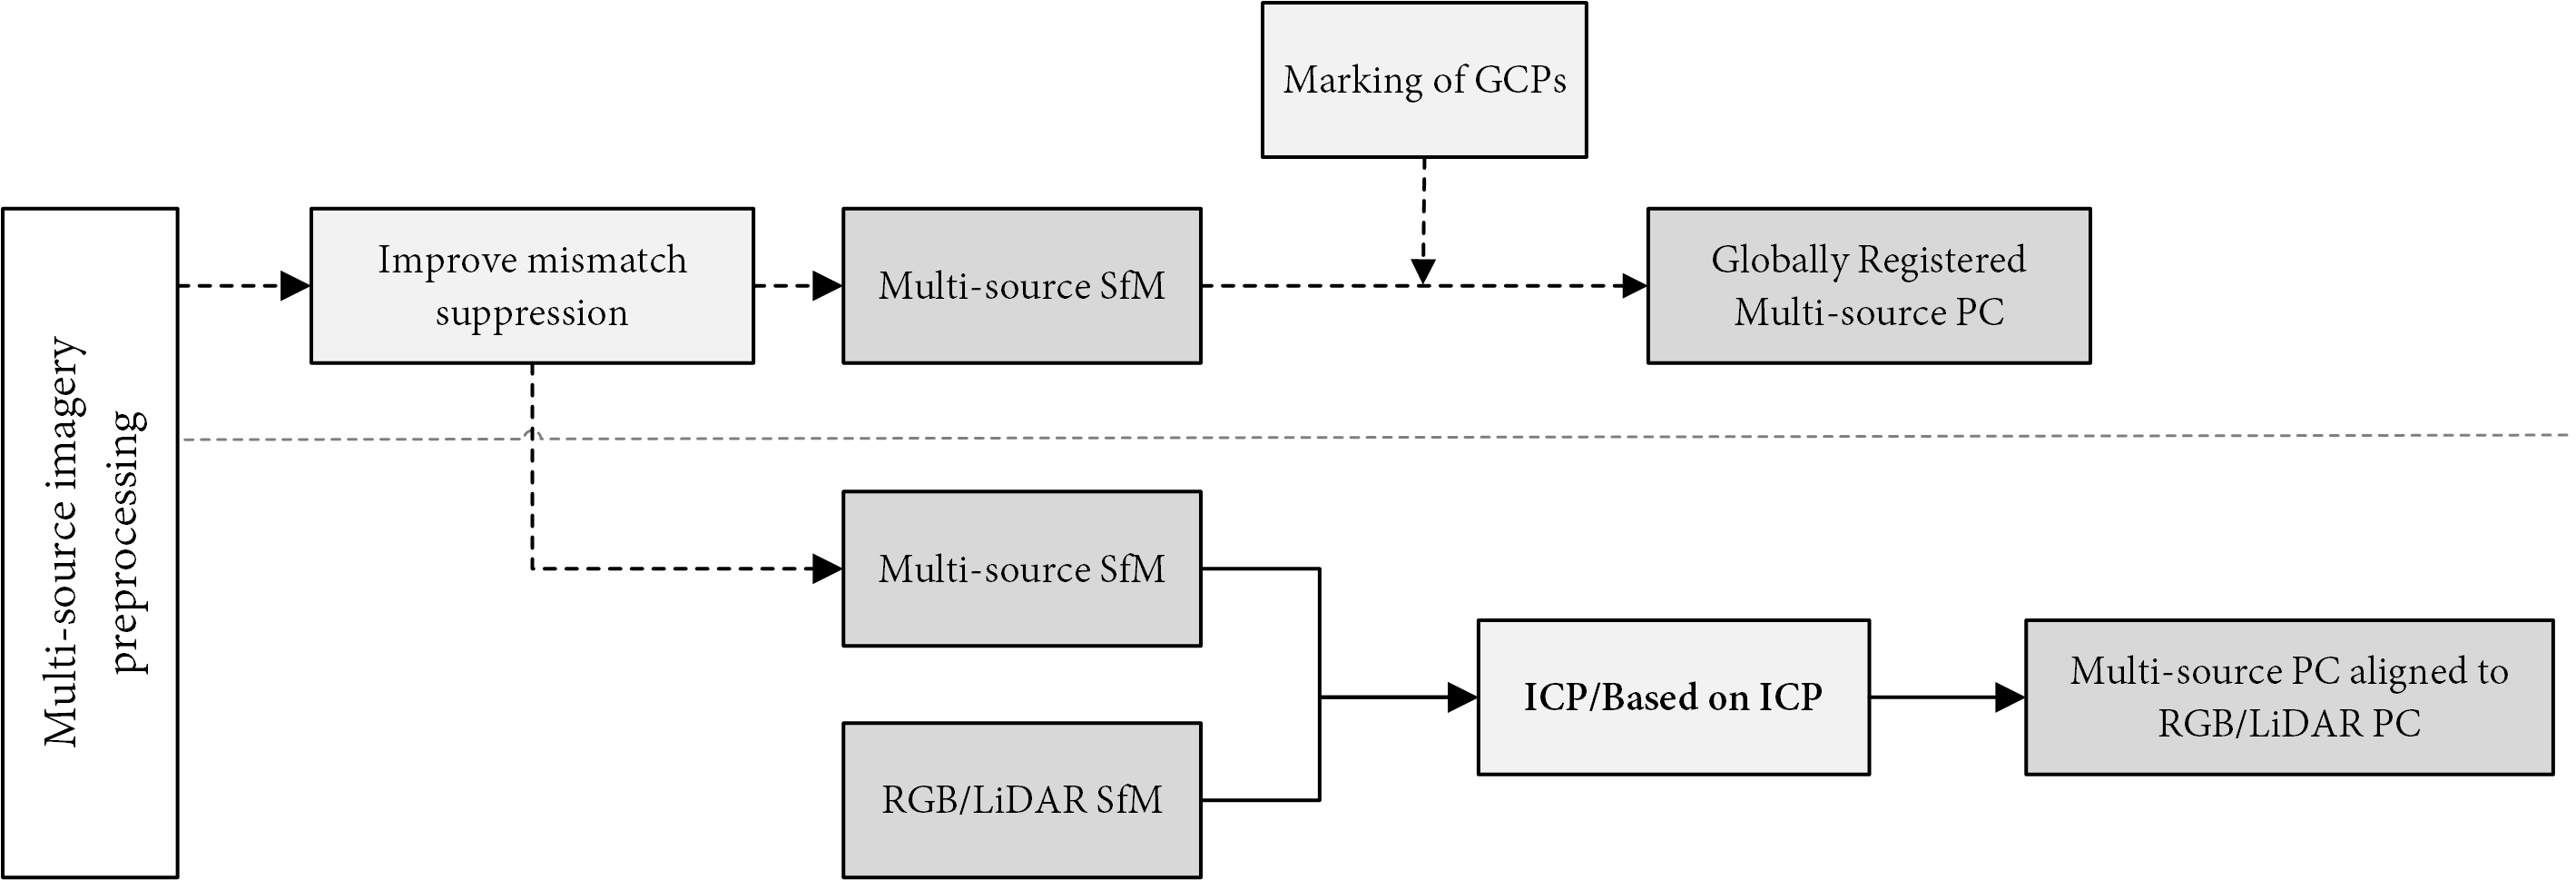
\includegraphics[width=\linewidth]{figs/context/fusion_01.png}
	\caption{Two methods for reconstructing 3D thermographic models. First, SfM algorithm is used over both kind of images, whereas in the second, a base point cloud is aligned with an alternative point cloud using rigid estimation processes. }
    \label{fig:fusion_data_01}
\end{figure*}

SfM has been extensively studied as a first step for 3D thermographic modeling \cite{dahaghin_precise_2021, dahaghin_3d_2019, gonzalez_thermal_2019, grechi_3d_2021, webster_three-dimensional_2018, sledz_thermal_2018, kniaz_thermal_2018, hoegner_mobile_2018, zheng_thermal_2020, guilbert_fusion_2020}. The main concern is that resulting point clouds typically lack point density for monitoring tasks. Besides this, obtaining valuable and precise point clouds also relies on accurate geopositioning. However, recognition and marking of GCPs to help with accurate geopositioning may not be trivial due to the low image resolution and colour contrast \cite{sledz_thermal_2018}. Consequently, SfM has been frequently followed by several refining operations, mainly by using other data sources that help on providing data that thermography lacks. Nevertheless, previous work has explored photogrammetric reconstructions along with the traditional marking of GCPs \cite{dahaghin_precise_2021, gonzalez_thermal_2019, zheng_thermal_2020, sledz_thermal_2018}. Boesch et al. \cite{boesch_thermal_2017} and Nishar et al. \cite{nishar_thermal_2016} overcome the limited visibility of GCPs in thermographic images by using metal-coated GCPs with low emissivity, in comparison with the surrounding vegetation. Two case studies using non-metal-coated GCPs are shown in Figure \ref{fig:gcps_thermography}, thus showing the difficulties in marking them on some kinds of scenery. The enhancement of the accuracy of External Orientation Parameters (EOP) has also been studied by replacing the EOP estimated from devices with higher precision (e.g., RGB devices) \cite{jo_dense_2021}.

\begin{figure}[!ht]
	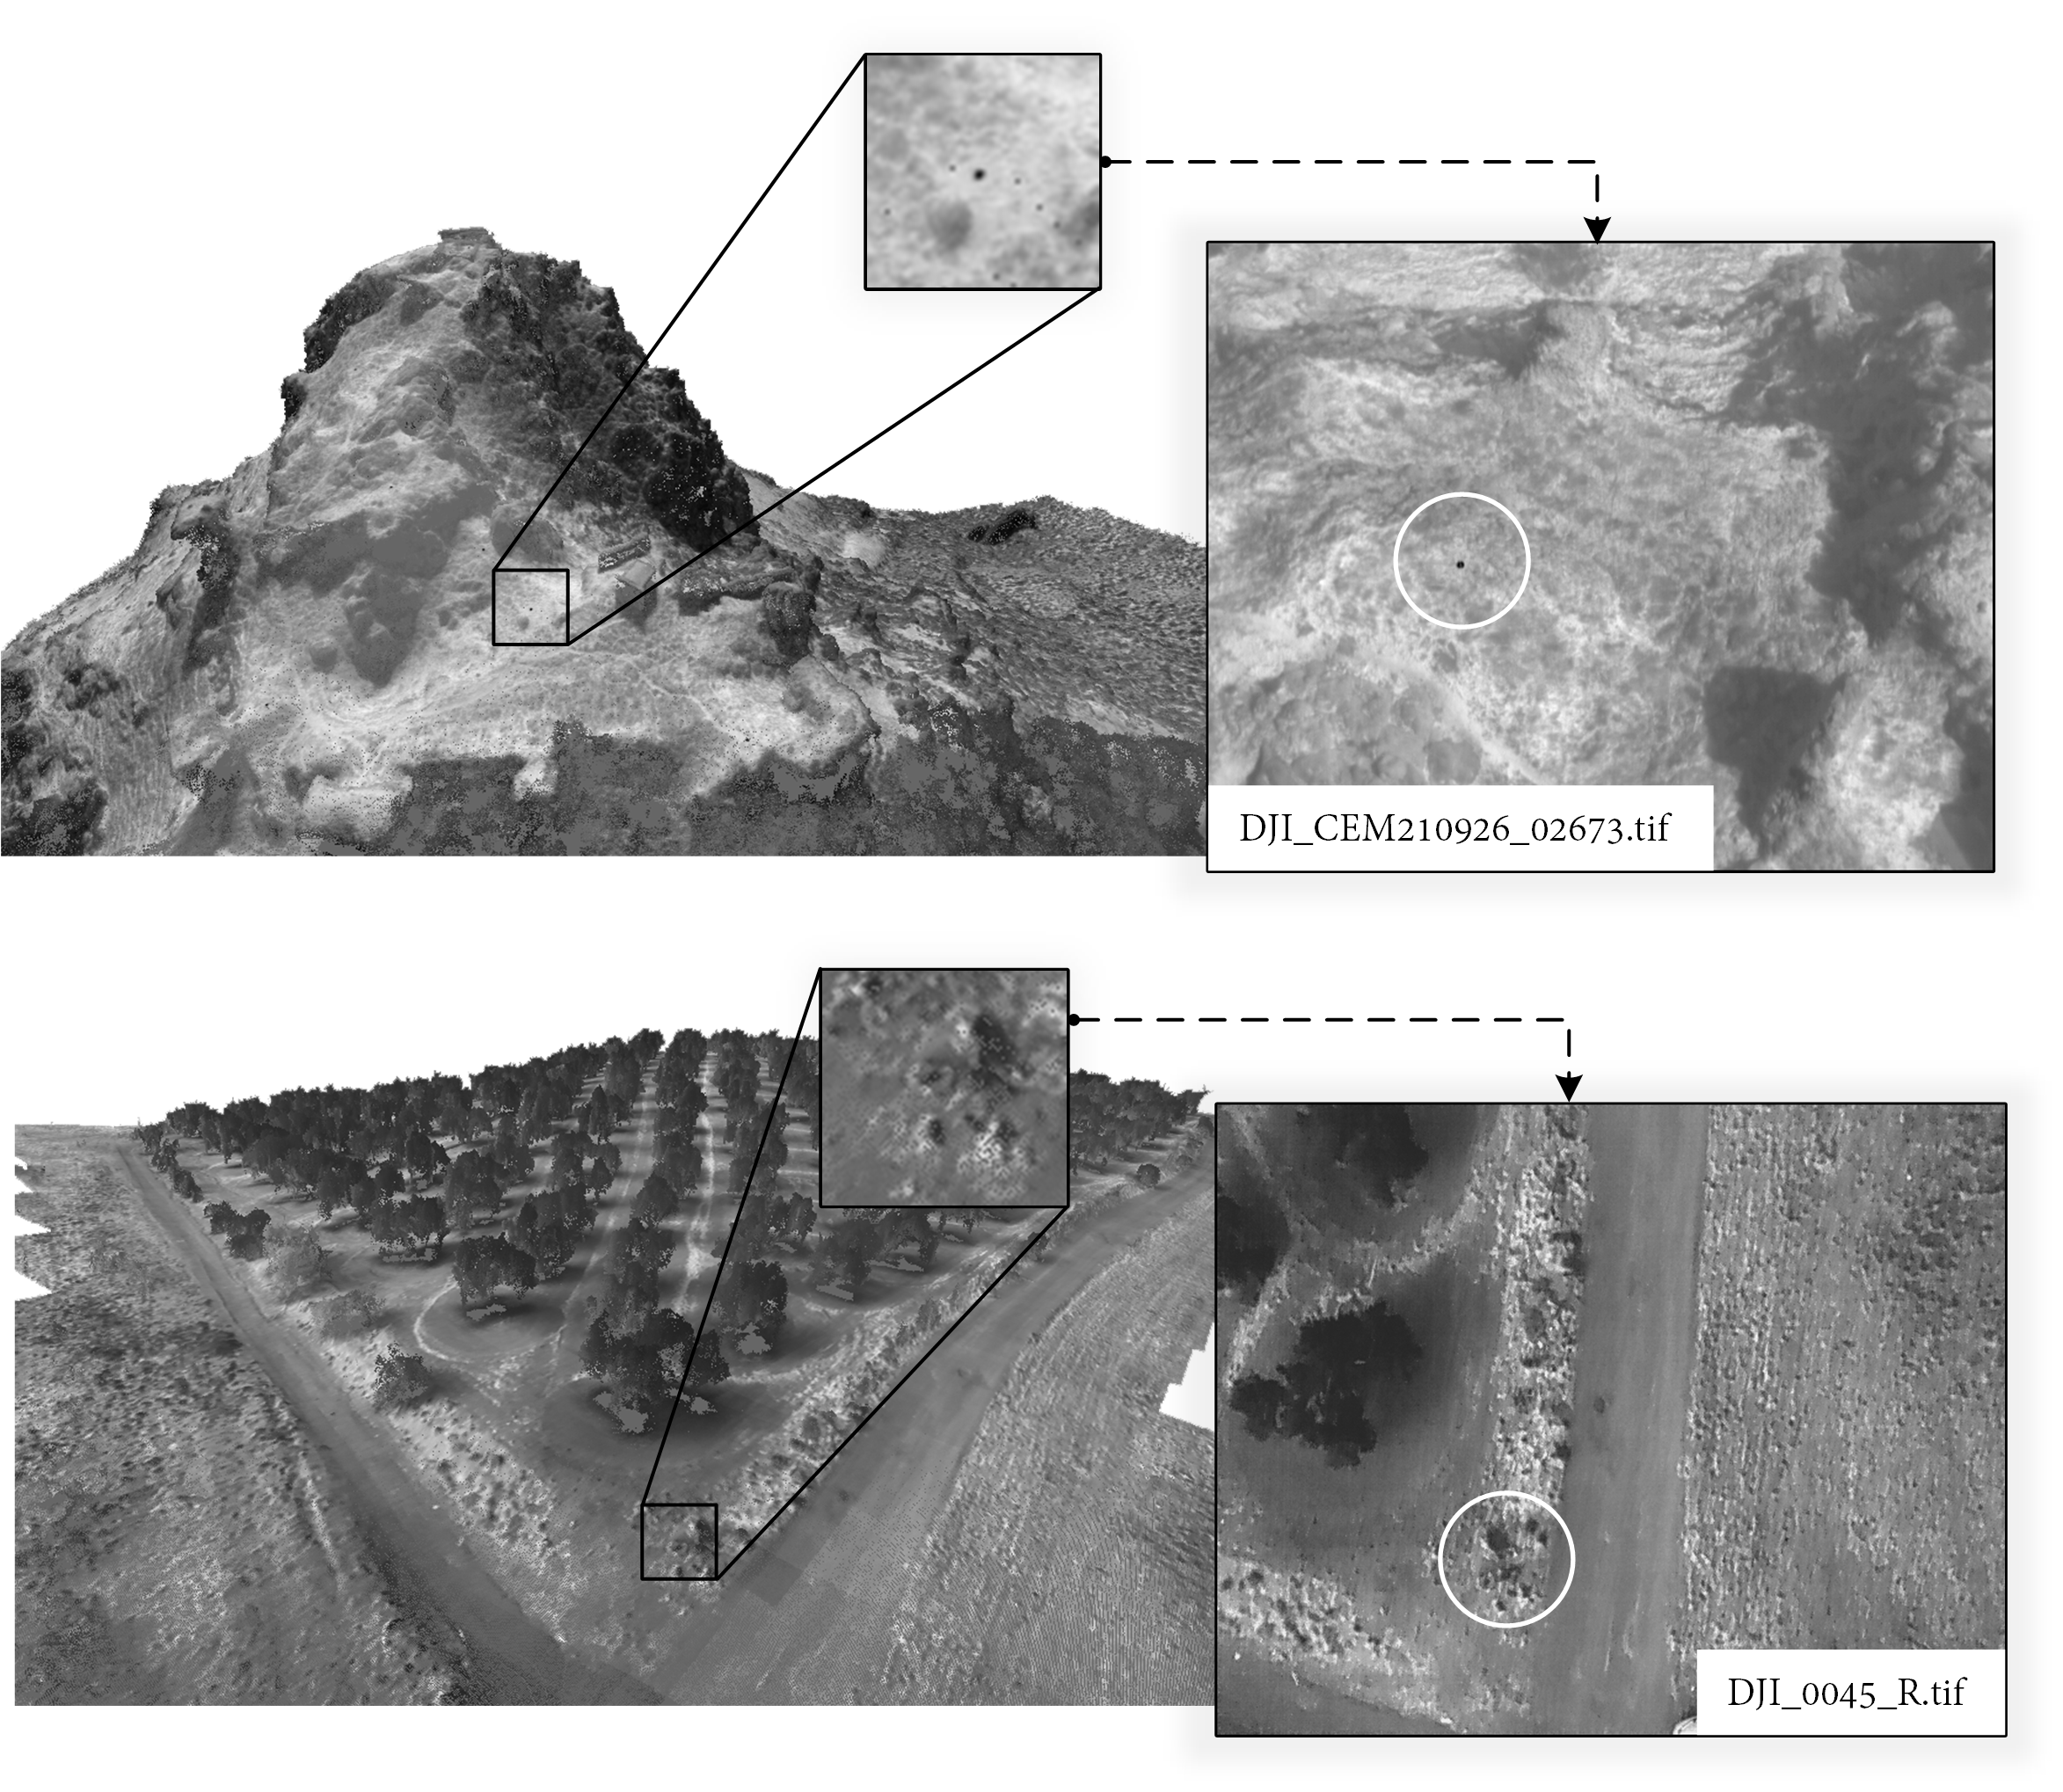
\includegraphics[width=\linewidth]{figs/context/gcps.png}
	\caption{Non-metal-coated GCPs made of plastic under different scenarios. In the latter, these are harder to mark as surrounding surfaces to the GCPs show a similar appearance. However, the GCP's material did not reach a temperature as high as the surrounding surfaces, and therefore, was notably more visible to the naked human eye. }
    \label{fig:gcps_thermography}
\end{figure}

Additionally, some preprocessing methods have been proposed for the optimization of photogrammetry. Maes et al. \cite{maes_optimizing_2017} estimated the thermal camera parameters using the Brown-Conrady distortion model. The temperature was corrected by decoupling the influence of air temperature throughout several flights, whereas improvements in image position were achieved considering the onboard GPS/GNSS log file. To overcome the limitations imposed by SfM keypoint detection, several studies propose alternative algorithms to enhance both feature extraction and suppression of mismatches. In this regard, Kong et al. \cite{kong_3-d_2018} discarded mismatches by applying first a K-Nearest Neighbor algorithm (KNN) to remove obvious false matches, followed by a modification of AC-RANSAC including the temperature as a constraint to discern mismatches. As opposed to the RANSAC algorithm, both procedures are not dependent on a threshold given by model hyperparameters. On the other hand, feature descriptors were altered when thermal imagery was merged with other data sources, e.g., RGB high-resolution imagery.

\subsubsection{3D reconstruction from multiple sources}

The fusion of several data sources along with thermography has been extensively investigated. RGB images are the main one since they present higher dimensionality and thus enable the generation of more accurate and dense 3D models. Therefore, the vast majority of previous work is based on the building of RGB point clouds and the subsequent projection/alignment of thermographic data \cite{hosoi_estimating_2019}. Registration of visible and thermal imagery has been traditionally performed through feature descriptors, either in 2D or 3D. Consequently, features that are visible on both spectral ranges are automatically matched, whereas mismatches are filtered out. At this point, both data sources are matched and 3D RGB points could be projected into thermal images. Methods based on projection, such as the one described, are able to generate larger point clouds with upsampled thermal information. 

From the wide range of work concerning the matching of visible and thermal imagery, some studies part from the assumption that both data sources fit perfectly with no further processing \cite{hou_fusing_2021, stojcsics_high_2018}. This scenario does not represent normal acquisition conditions; instead, visible and thermal imagery may record slightly different areas due to the delay between non-simultaneous camera recording, the platform's movement and device calibration, which may degrade over time. The same shortcomings remain even for co-acquired visible and thermal imagery, such as in the Zenmuse XT2 sensor. Accordingly, images can be registered by finding a transformation matrix that is able to describe the difference between them, e.g., affine and homography matrices. 

\begin{figure*}[!ht]
	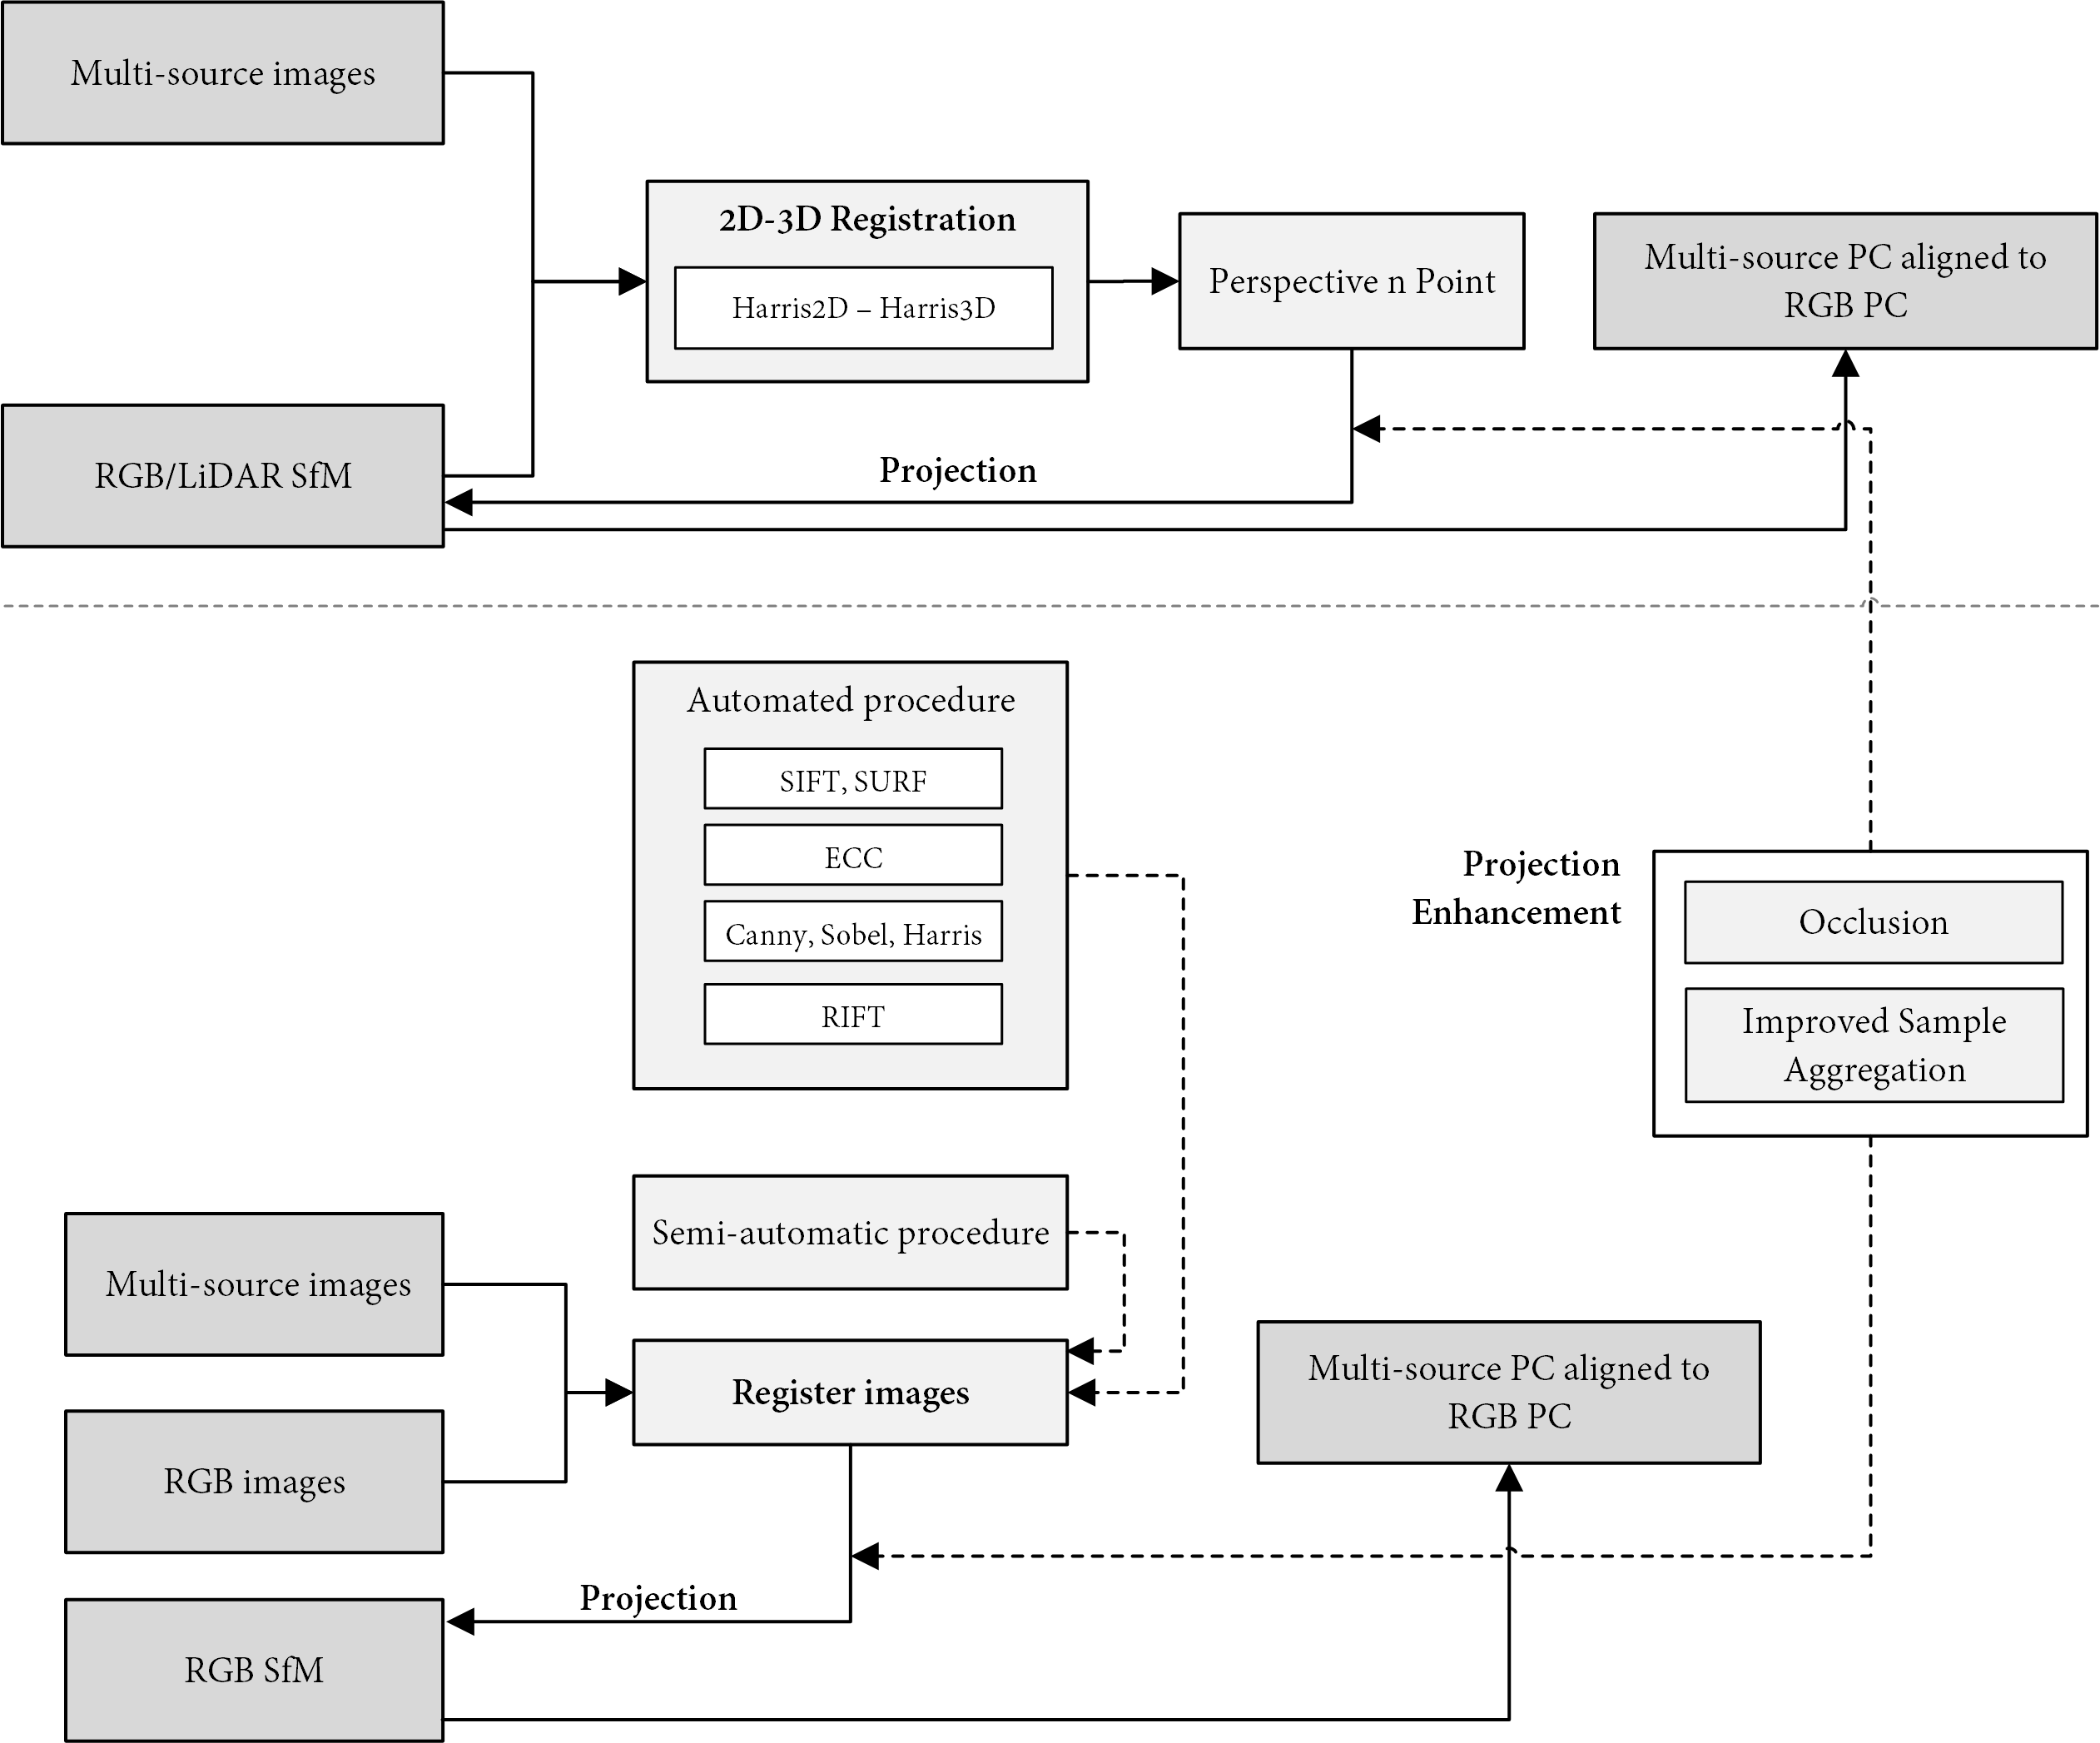
\includegraphics[width=\linewidth]{figs/context/fusion_03.png}
	\caption{Two methods for reconstructing 3D thermographic models. First, SfM algorithm is used over both kind of images, whereas in the second, a base point cloud is aligned with an alternative point cloud using rigid estimation processes. }
    \label{fig:fusion_data_03}
\end{figure*}

Instead of using colourimetric data, other proposals focus on the calibration of a multi-sensor system. Thermographic imagers are frequently combined with RGB cameras \cite{javadnejad_photogrammetric_2020, landmann_multimodal_2019, adan_fusion_2017} and LiDAR \cite{adan_fusion_2017, hoegner_fusion_2018}. Co-registration of dual-sensor systems was performed by estimating the translation (lever-arm) and rotation (boresight) matrices that represent the relative differences between both sensors (Figure \ref{fig:fusion_data_04}). To this end, the calibration is performed by using semi-automatic or manual identification of features visible on any pair of images. Regardless of the correctness of this approach, this pre-calibration was proven to perform worse in inexpensive, consumer-grade thermal cameras \cite{javadnejad_photogrammetric_2020}. Javadnejad et al. \cite{javadnejad_photogrammetric_2020} explained that constructing a checkerboard calibration panel is harder for thermography, plus the lack of sharp edges leads to mediocre estimations. In any case, if the matching transformations are known either in 2D or in a dual-head system, RGB pixels can be projected into thermal imagery. Finally, larger point clouds can also be generated by mixing both RGB and thermal imagery during the SfM's BA phase, followed by the generation of a dense point cloud that only integrates RGB data. As a result, thermographic data is described with respect to RGB data by means of Scale-invariant feature transform (SIFT) features and the point cloud can be subsequently projected into thermal images \cite{hoegner_3d_2016}. As a counterpart, this approach relies on SIFT operator to be able to find feasible features over images with different radiometric behaviour. 

\begin{figure*}[!ht]
	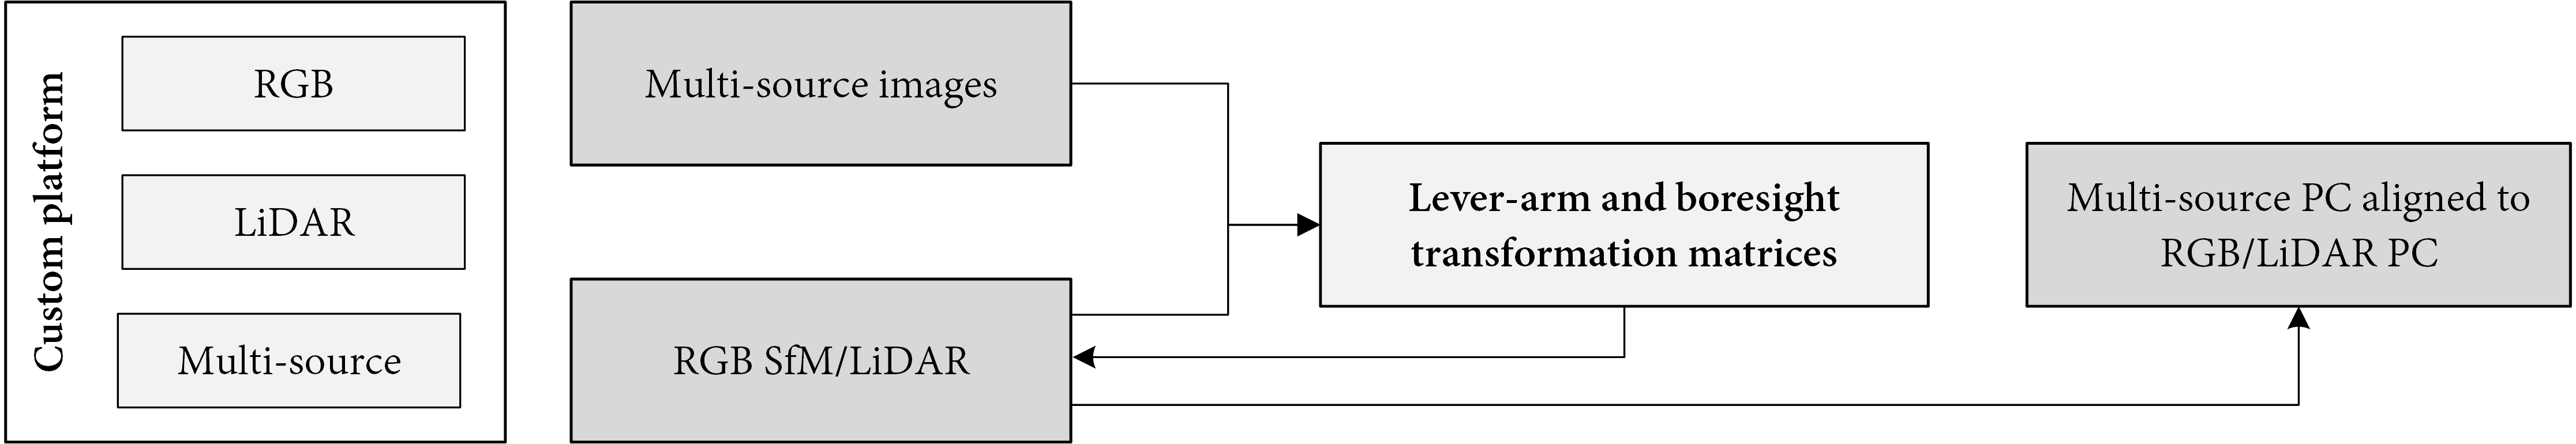
\includegraphics[width=\linewidth]{figs/context/fusion_04.png}
	\caption{Multi-sensor system is calibrated with the aim of projecting imagery into a sole coordinate system.}
    \label{fig:fusion_data_04}
\end{figure*}

The overall procedure on image registration is shown in Figure \ref{fig:fusion_data_03}. The main challenges concerning feature descriptors are in the selection of one of them. From the reviewed literature, edge-based detectors were preferred over conventional descriptors such as SIFT or Speeded-Up Robust Features (SURF). Canny and Sobel filters have been previously applied to contour detection \cite{hoegner_3d_2016, hoegner_evaluation_2016}. The resulting contours were also filtered out to extract only prominent edges through Hough transform \cite{hoegner_evaluation_2016}. These solutions were adopted to overcome SIFT drawbacks for imagery with different radiometric data. Yet, these solutions barely work in forestry and agricultural environments since vegetation edges are not relevant enough nor distinguishable for matching features (Figure \ref{fig:feature_detection}). Previous work has also described matching algorithms on the frequency domain to handle nonlinear radiation differences in thermography and visible imagery, such as Radiance Invariant Feature Transform (RIFT) \cite{lin_fusion_2019}. Feature matching methods could also be followed by techniques to suppress mismatches, such as RANSAC \cite{lin_fusion_2019}.

\begin{figure*}[!ht]
	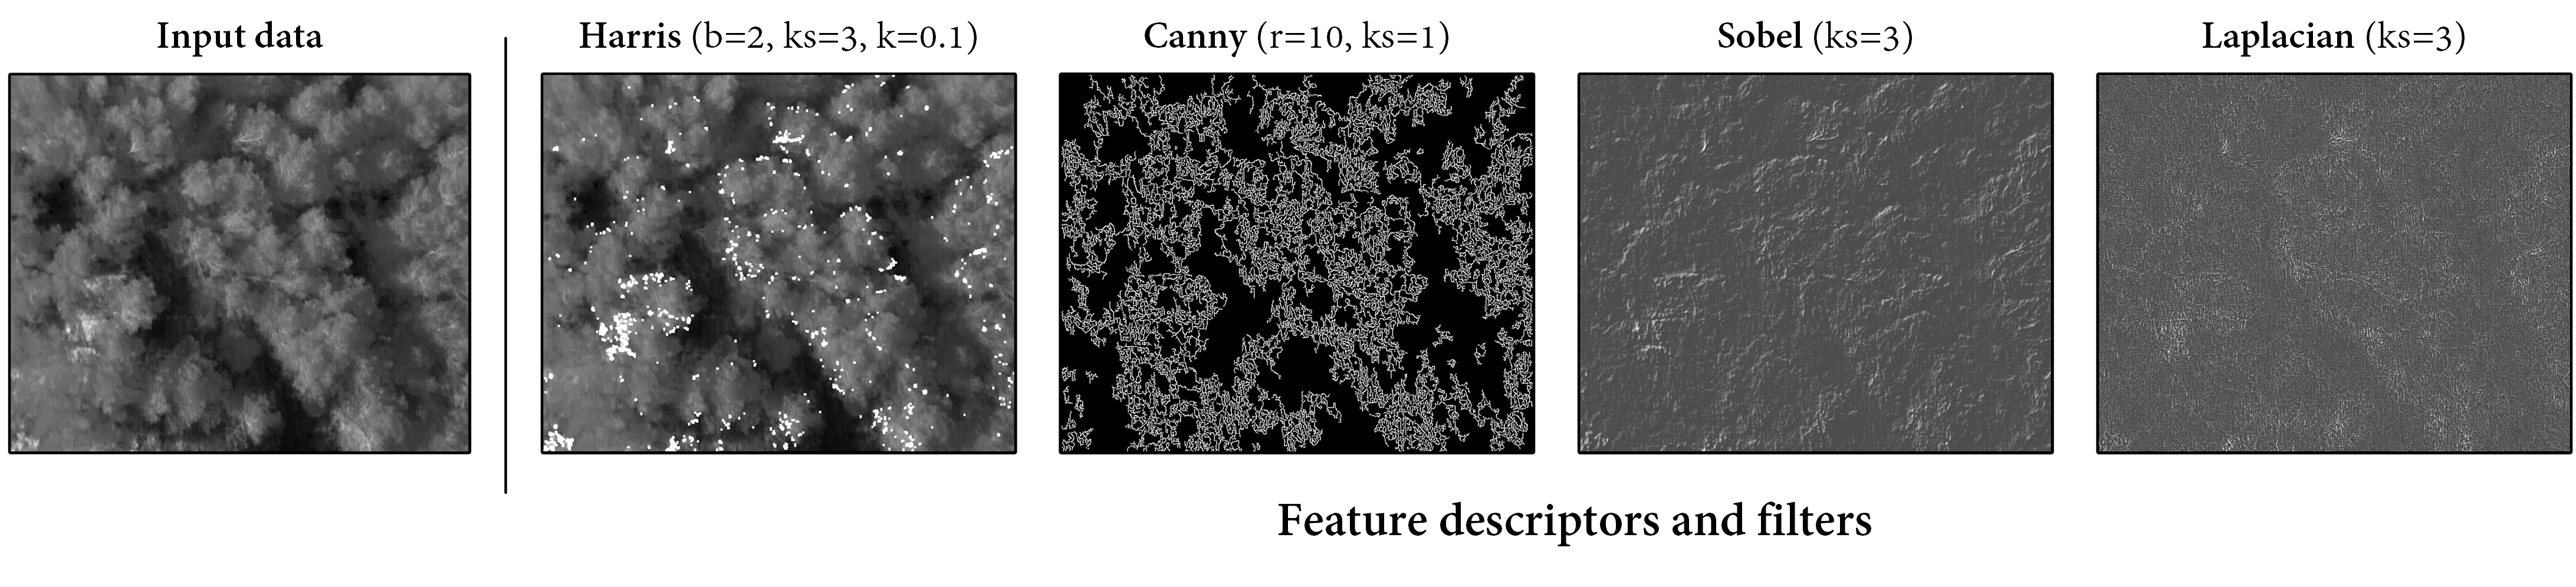
\includegraphics[width=\linewidth]{figs/context/feature_detection.png}
	\caption{Comparison of edge-based descriptors that serve as the core for registration algorithms in the literature. For vegetation, these are less likely to work as no relevant features are found. $\textit{ks}$ refers to kernel size, the ratio is presented as $\textit{r}$, and $\textit{k}$ is a free parameter on the Harris detector. The brightness of the two first images is increased to improve the visualization.}
    \label{fig:feature_detection}
\end{figure*}
% Fig. 8. Comparison of the core of several registration algorithms. Edge-based descriptors are shown as insufficient methods for environments with dense vegetation, while methods not dependent on a linear gradient, such as ECC, are proved to perform better. ks refers to kernel size, the ratio is presented as r, and k is a free parameter on the Harris detector. The brightness of the two first images is increased to improve the visualization.
  
Supervised procedures have been proposed by manually matching RGB and thermal points. Ham and Golparvar-Fard \cite{ham_automated_2013} estimated the epipolar geometry between both camera systems by manually picking image features, whereas \cite{huang_combining_2018, macher_combination_2019} were helped on this task with checkerboard images and relevant image key-points, e.g., building corners. Lafi et al. \cite{lafi_3d_2017} performed semi-automatic stitching of thermal images by marking relevant features on thermal images, thus generating a panoramic image that was finally mapped to a 3D RGB point cloud. However, semi-automatic registration is time-consuming and hard to apply over large datasets. Indeed, this procedure is more appropriate for generating thermographic models from a few images, rather than big datasets. 

Projection can also be performed by mixing 3D products and thermal imagery. For that purpose, the Perspective n Point (PnP) optimization problem is solved by pairing 3D and 2D features, thus estimating the cameras' pose. Most of these features are extracted through edge-based operators. Furthermore, SIFT and SIFT3D descriptors have been reported to identify an insufficient number of key points. Hence, contour-based approaches have frequently exchanged the traditional SIFT descriptor by Harris and Harris3D operators \cite{zhu_fusion_2021, zhu_direct_2019}. Harris3D has been described as a robust method whose detected features are less likely to appear in other locations within a single image. Instead of considering contours as significant features, Lin et al. \cite{lin_fusion_2019} proposed to use the line intersections as key points. Nevertheless, there is seldom a robust method to accurately match 2D and 3D features. Therefore, the matching ends up being supported by human operators \cite{zhu_fusion_2021, zhu_direct_2019} or by restricting the search space through GPS/GNSS data, along with RANSAC to discard mismatches \cite{lin_fusion_2019}. 

Reconstructing and coregistrating thermal and visible point clouds is also tempting in spite of the density and noise gap among them. This approach is suitable for thermographic reconstructions with sufficient density and quality. Difference minimization between two point clouds could be performed through Iterative Closest Point (ICP) by estimating the composite matrix of translation, rotation, and optionally, scaling \cite{hoegner_mobile_2018, webster_three-dimensional_2018, clarkson_thermal_2017}. Rather than solely applying the ICP algorithm, thermal point clouds could be preprocessed by applying noise filtering and a coarse global registration through a rigid body transformation using the cameras' pose \cite{truong_registration_2017}. Yet, ICP may be used as a local registration for further improving the alignment. An alternative to ICP is Fast Global Registration (FGR), which is proven to achieve better results for noisy datasets \cite{lin_fusion_2019}. Point clouds can also be registered by means of at least three GCPs whether they can be accurately identified on thermographic reconstructions \cite{dahaghin_3d_2019}. In addition, the use of ICP along with KNN has been investigated to assign thermal data to RGB points, whose output is a dense 3D model with upsampled thermal information. Recently, equivariant descriptors have been proposed by extracting features icosahedral groups, thus achieving rotation invariance \cite{wang_you_2022}.

\begin{marginfigure}[.15cm]
	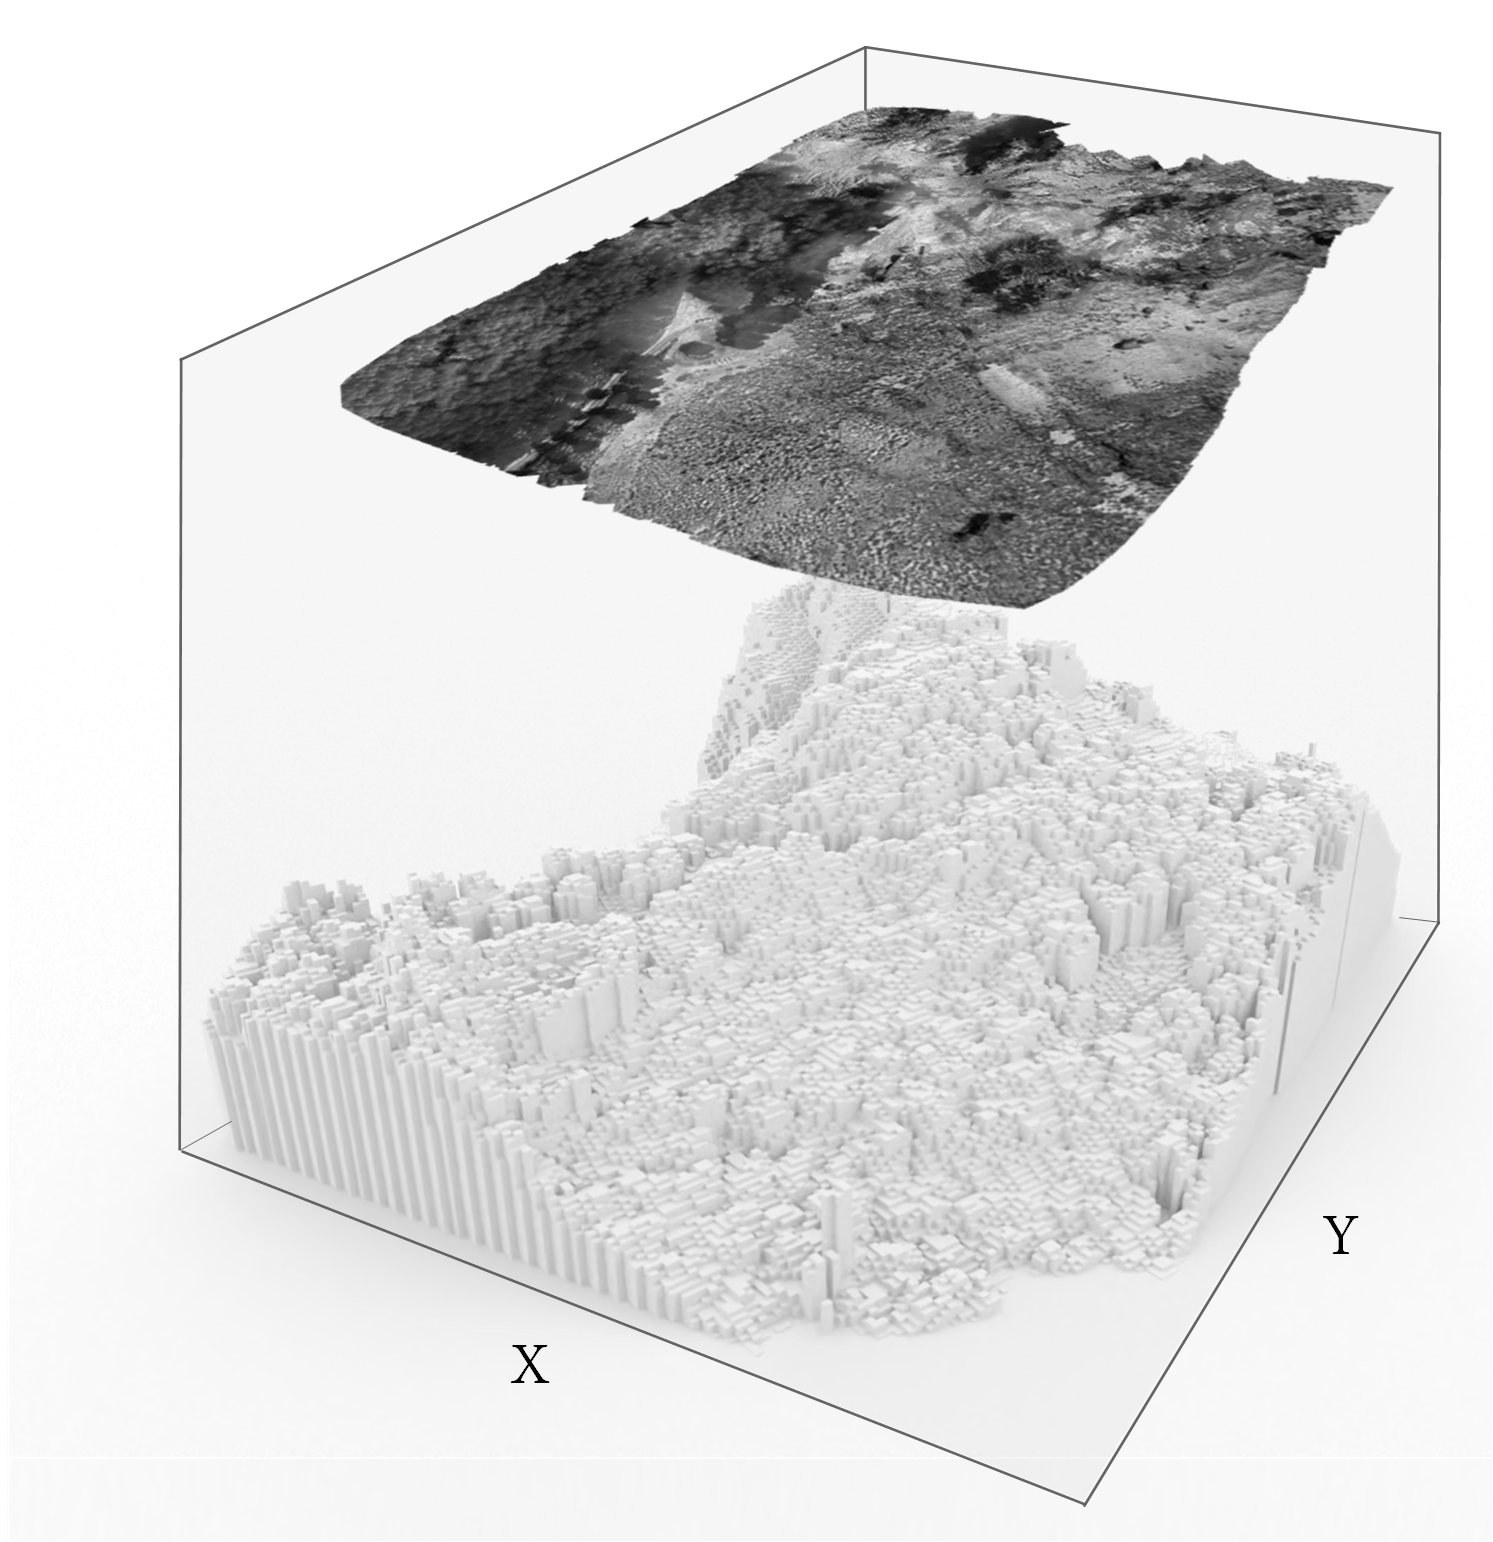
\includegraphics{figs/context/orthomosaic_projection.png}
	\caption{Projection of orthomosaic (top map) over a 2.5D heightfield from the voxelization of a point cloud.}
	\label{fig:ortho_projection}
\end{marginfigure}
Thermographic 3D models can also be built by combining LiDAR and visible point clouds with thermal maps placed in the same coordinate system (Figure \ref{fig:fusion_data_02}). Comba et al. \cite{comba_2d_2019} fused an RGB point cloud with a coregistered thermal orthomosaic, whereas Adán et al. \cite{adan_towards_2020} combined LiDAR results with 360-degree maps of thermographic information. Hence, this approach relies on the generation of a thermal composition with limited resolution and its projection in a 3D model. Results are not 3D point clouds, but heightfields (2.5D) where thermal data is assigned to stacks \cite{juszczyk_wound_2021}. Therefore, these results are more likely to present occluded areas without analyzable data. Adán et al. \cite{adan_towards_2020} overcame this challenge through a mobile scanning platform and the joining of multiple thermal point clouds using the platform odometry and the ICP algorithm. 

\begin{figure}[!ht]
	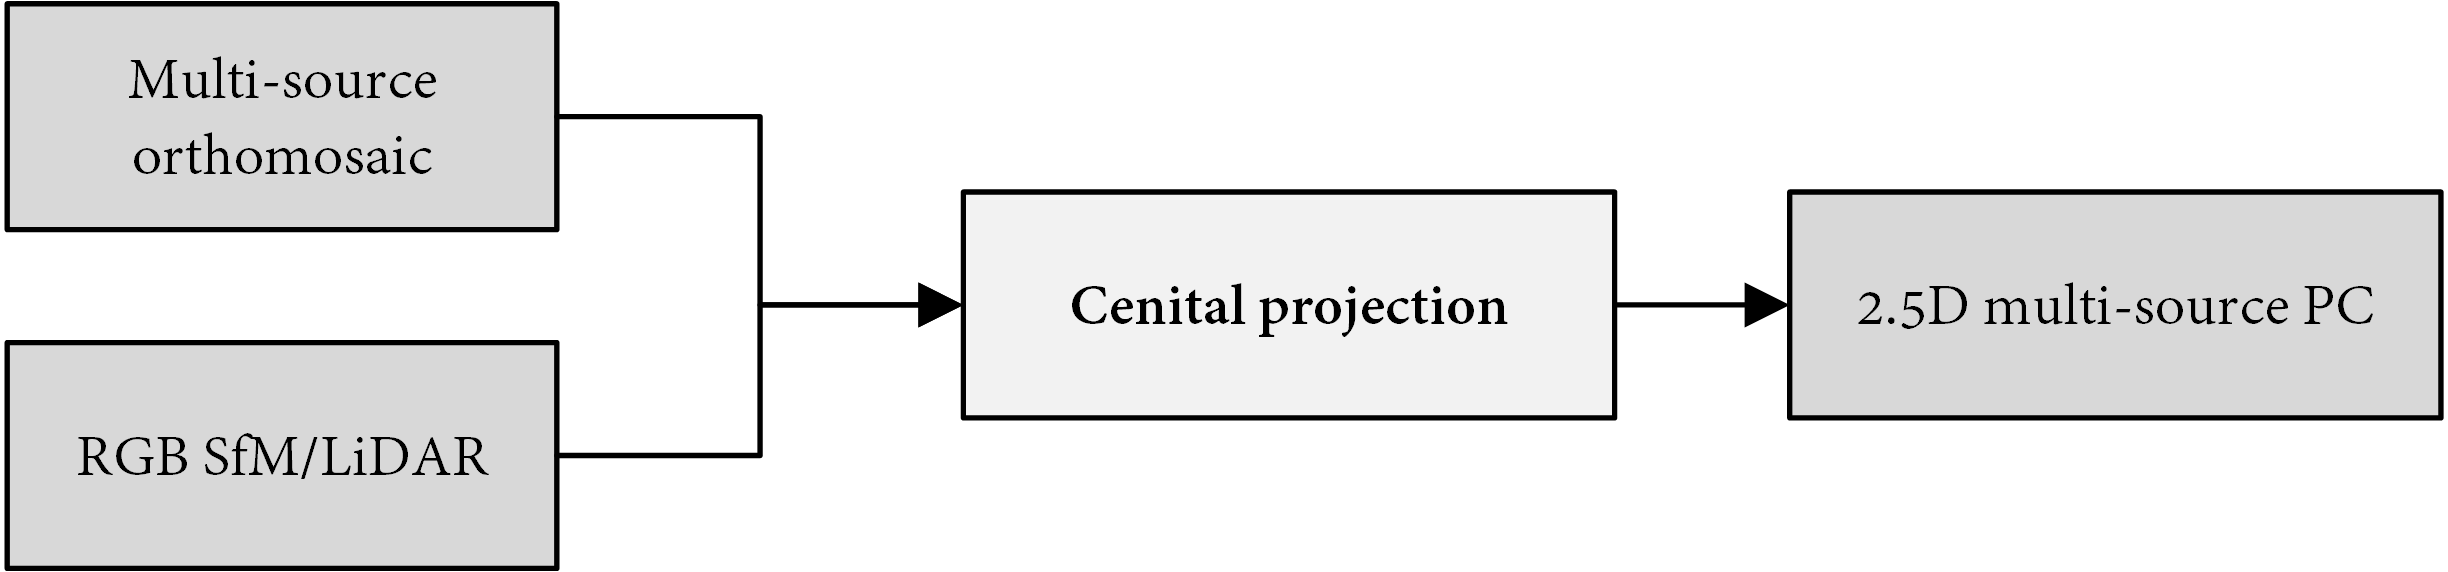
\includegraphics[width=\linewidth]{figs/context/fusion_02.png}
	\caption{2.5D point clouds are generated by projecting the orthomosaic of an alternative data source over a baseline point cloud.}
    \label{fig:fusion_data_02}
\end{figure}

\subsection{Fusion of multispectral imagery}

The generation of 3D multispectral data is possible due to a high increase in image quality and resolution provided by recent acquisition systems. The 3D representation of reflectance distribution along the model surface allows us to develop a more detailed inspection and analysis of plant health. Thus, self-occluded features can be revealed by being observed from multiple viewpoints and represented on a 3D model. According to previous studies focused on the 3D reconstruction of multispectral imagery, two main categories are described considering the data acquisition system: satellite-based and UAV-based imagery. Main techniques and popular sensors are reviewed to pose a general overview of existing solutions for the generation of 3D multispectral models.

Traditionally, most of the previous work is based on satellite image mapping on 3D photogrammetric point clouds and LiDAR models for monitoring the forest structure \cite{bolton_optimizing_2020, lechner_applications_2020}, multitemporal observation of crops \cite{gadiraju_multimodal_2020, qadeer_spatio-temporal_2021} and semantic segmentation of urban and natural scenarios \cite{ballouch_toward_2022, saralioglu_semantic_2020}. State-of-the-art reconstruction methods from satellite data typically generate elevation data. Over the last few years, promising studies have focused on the super-resolution of satellite images through different deep-learning approaches \cite{gomez_experimental_2022, stucker_resdepth_2022}. Consequently, the cited advances and modern high-resolution satellite sensors allow us to recover full 3D surfaces from multi-view satellite panchromatic images \cite{han_state_2020, rothermel_photometric_2020}. Digital surface models can be efficiently modelled with automatic image matching from multiple optical stereo images, which are acquired in the same orbit \cite{gui_automated_2021, qin_critical_2019}. The resulting 3D meshes or point clouds can be directly fused with multispectral bands of satellite imagery. According to the satellite's capabilities to produce 3D multispectral data, the most recent studies only produce digital elevation models (DEM) enriched by spectral attributes to enable a more comprehensive characterization and view of the surveyed area \cite{dalponte_mapping_2020}, \cite{sagan_field-scale_2021, wang_extraction_2020}. Thus, real-world 3D scenarios can be labelled and this data provides a high interest for many environmental applications. In fact, to increase the size of current multispectral satellite image sets, recent work is focused on Generative Adversarial Networks (GANs) for the generation of synthetic multispectral satellite images \cite{abady_gan_2020, mohandoss_generating_2020}. These techniques enable obtaining labelled synthetic imagery that can be mapped on 3D scenarios in data-scarce regions.

Multispectral imagery is composed of several broad bands that may not correspond to the same target area. This occurs due to the sensor architecture, as each band requires a different lens placed at different locations within the platform. Platform, calibration of each individual imager deteriorates over time and therefore, their optical parameters differ from the manufacturing ones. Shen et al. \cite{shen_multi-modal_2014} introduced an image-matching solution based on a descriptor measuring the degree of matching for every pixel. Other works used the image metadata to correct the misalignment \cite{jhan_band--band_2016, jhan_investigation_2017} relies on, while \cite{jhan_investigation_2017} included parameter estimating methods such as Random Sample Consensus (RANSAC) to minimize the error induced by calibration uncertainty. Supervised models are also revised based on image-matching and metadata approaches in a supervised model.

Digital surface modeling may be performed by UAV photogrammetric reconstruction using multispectral imagery. James et al. \cite{james_uav_2021} highlighted the contribution of infrared channels (NIR and Red-Edge) compared to the visible ones for the XYZ accuracy in the digital surface model (DSM) reconstruction over the coastal fringe. 3D points are usually reconstructed using images in every single spectral band. Speeded up robust features (SURF) algorithms \cite{sedaghat_high-resolution_2019} and Scale-invariant feature transform (SIFT) algorithms \cite{saleem_robust_2014} are commonly applied for feature detection and feature matching. According to previous studies that summarized the results of aerial image registration \cite{tsai_accelerated_2017}, the SIFT method outperformed other algorithms in terms of quality of results and runtime. In this scope, Matese et al. \cite{matese_assessment_2017} presented an assessment of the canopy height model in a vineyard using UAV-based multispectral imaging, Liu et al. \cite{liu_registration_2018} proposed a method for multispectral 3D points registration and plant inspection and Zainuddin et al. \cite{zainuddin_3d_2019} discussed the multispectral camera capabilities to acquire 3D data. The extracted tie points were generated using SfM, which were then used as input to generate a dense point cloud based on the multi-view stereo (MVS). 

\begin{figure}[!ht]
	\includegraphics[width=\linewidth]{figs/context/feature_extraction.png}
	\caption{Comparison of two traditional feature descriptors and matching algorithms: SIFT and ORB (Oriented FAST and rotated BRIEF). In this example, both are used to match multi-view sequences of the same scene.}
    \label{fig:feature_descriptors}
\end{figure}

UAV multispectral images have enough resolution to directly generate photogrammetric point clouds, which may be upsampled later \cite{qian_pu-gcn_2021}. Still, other work is focused on mapping multispectral image over 3D models from LiDAR sensors or RGB imagery. In the following paragraphs, recent work is presented considering: (1) image-based methods, and (2) LiDAR-based solutions for the generation of 3D multispectral data. Recently, Jurado et al. \cite{jurado_multispectral_2020} proposed a novel pipeline to generate dense multispectral point clouds by mapping multispectral images on dense point clouds which were reconstructed using high-resolution RGB images. Firstly, a sparse point cloud is reconstructed using NIR images. This 3D model is then aligned with the RGB model and the resulting transformation is applied for each multispectral camera. Thus, a unique reference system is set and then, every multispectral image is mapped on the RGB point cloud considering the occlusion problem. Since multispectral images have a lower resolution than RGB images, the K-Nearest Neighbor algorithm is used for resampling to obtain spatially matched multispectral and RGB 3D models. With this solution, dense point clouds with multispectral attributes can be generated. Other studies focused on generating multispectral point clouds with aerial photogrammetry. Comba et al. \cite{comba_unsupervised_2018} detected vineyards from 3D point-cloud maps, generated from UAV multispectral imagery. Shen et al. \cite{shen_estimation_2019} generated point clouds from UAV multispectral and RGB images for the estimation of forest structural attributes. Villacrés et al. \cite{villacres_construction_2022} proposed the reconstruction of 3D maps of vegetation indices retrieved from UAV multispectral imagery in forestry areas. Moreover, other approaches are based on multispectral image registration on 3D point clouds using RGB-D sensors that can be embedded on aerial and terrestrial platforms. Clamens et al. \cite{clamens_real-time_2021} implemented a method based on feature-based and corner-based registration approaches to register images from the RGB-D camera with multispectral images. The combination of multispectral, RGB and depth images generates a multi-modal data fusion, which allows the extraction of several types of information from the environment.

Regarding other studies that use multispectral 3D data, the integration of LiDAR and multispectral sensors is a well-known solution. Initially, these acquisition systems were quite heavy and coupled to an aircraft. Previous work was developed for forest structure characterization \cite{manzanera_fusion_2016} and urban scene classification \cite{guo_relevance_2011}. Data fusion was carried out by the back-projection method, proposed by Valbuena et al. \cite{valbuena_integrating_2014}. Back-projecting consists in rendering LiDAR from the optical camera’s perspective in order to obtain the pixel information that corresponds to each return. Then, the pixel attributes are fetched and retrieved to the original position of LiDAR returns, and these are effectively textured. This projection is developed considering information about the optical sensor architecture (internal parameters) and the platform position and bearing (external parameters). The collected multispectral data are usually transformed from Digital Numbers (DNs) values to both reflectance and several vegetation indices. Multispectral data along with the more traditional LiDAR height metrics are beneficial for predicting variables describing forest structural heterogeneity \cite{valbuena_most_2018} and for improving public data through a building segmentation from Convolutional Neural Networks (CNNs) \cite{griffiths_improving_2019}. 

In recent years, the proliferation of light-weight LiDAR sensors allows a physical integration of a multispectral camera and LiDAR sensor coupled to a UAV. In this way, simultaneous data can be acquired with a greater spatial resolution. Both sensors usually use the same GPS-IMU configuration to avoid the registration challenges caused by time-space inconsistency. Despite both sensors being mounted on the same platform, multispectral data must be calibrated following two main steps: (1) band-to-band multispectral image registration and (2) radiation correction model to solve the vignette effect. In this context, significant advances have been made focused on multi-sensorial data fusion. Sankey et al. \cite{sankey_quantifying_2021} proposed a novel methodology for UAV multispectral, hyperspectral and LiDAR data fusion in shrub-encroached desert grassland. However, this study is based on a comparison between 2D data using orthomosaics that are generated by Pix4D software (Pix4D SA, Lausanne, Switzerland), in the case of multispectral imagery, and SpectralView software (Headwall Photonics, Inc, Bolton, USA), in order to corregister the hyperspectral swatches. Gu et al. \cite{gu_uav-based_2020} carried out a method to integrate UAV multispectral data and LiDAR models. This is based on an inner relationship between the multispectral grid pixel and the unorganized point cloud from the LiDAR sensor. To infer a model from 2D images to 3D physical world two components are considered: reflectance and shading. 

The typical workflow of the proposed techniques involves the generation of a multispectral orthomosaic and then, an orthogonal projection is developed on 2.5D models. As shown in Figure 5, orthomosaics are generated using either thermal, multispectral or hyperspectral images. However, the mosaicking process usually generates some misalignment areas derived from positioning errors. In addition, measured data are interpolated representing many viewpoints as one ortho-pixel.

\subsection{Fusion of hyperspectral imagery}

For each pixel in an image, a hyperspectral sensor acquires the light intensity (radiance) for a large number (typically a few tens to several hundred) of contiguous spectral bands. Every pixel in the image thus contains a continuous spectrum and can be used to characterize the objects in the scene with great precision and detail. Typically, four approaches can be used for acquiring hyperspectral imagery (HSI) in remote sensing. However, the vast majority of sensors used in UAVs are classified as push-broom or snapshot. Since datacubes have a higher dimensionality than the two-dimensional (2D) detector arrays currently used in RGB and multispectral sensors, system designers must resort to either measuring time-sequential 2D slices of the cube (push-broom) or simultaneously measuring all elements of the datacube by dividing it into multiple 2D elements that can be recombined into a cube in post-processing. Figure \ref{fig:hyper_sources} illustrates the main principles behind push-broom and snapshot approaches.

\begin{figure*}[!ht]
	\includegraphics[width=\linewidth]{figs/context/hyper_sources.png}
	\caption{Pre-calibration of sensors helps on the projection of multi-source images over a point cloud.}
    \label{fig:hyper_sources}
\end{figure*}

Push-broom sensors include an input aperture (a long slit). A set of 2D detectors is used, so that all points along the line represented by the slit are sampled simultaneously. To form the complete 2D image of the area of interest, the sensor is moved in the direction orthogonal to the slit. In the specific case of this review, the UAV that carries the sensor plays this role. The array of detectors is pushed along the flight direction to scan the successive lines, and hence the name push-broom. Instead of a line scanner, the snapshot approach allows simultaneous recording of spatial and spectral information. This type of sensor enables the acquisition of a complete spectral data cube in a single integration, generating images from the areas of interest. This approach allows to directly acquire data, which reduces the post-processing complexity to obtain a 3D data cube. 

It is worth noting that the type of sensor greatly affects field operations, processing performance and the quality of the final product. More information regarding hyperspectral technology can be found in Adão et al. \cite{adao_hyperspectral_2017}. UAV-based hyperspectral technology continues to be developed. The fact that it allows us to obtain information in hundreds of adjacent narrow bands, will enable the acquisition of more complete information about the imaging scene, material or phenomenon. The fusion of different types of data with 3D information, regarding agricultural and forest applications, is the main focus of this review. Considering hyperspectral data and 3D information fusion, it would provide a more accurate scene understanding. This would also allow the development of unsupervised automatic sampling of meaningful material classes from the target area exploring new machine learning approaches. 

Methods to compute 3D hyperspectral models were proposed in close-range applications. For instance, Zia et al. \cite{zia_3d_2015} developed a method that applies SfM to images from different wavelengths and a 3D registration method to combine band-level models into a single 3D model. Kim et al. \cite{kim_3d_2012} described a system prototype composed of a laser sensor and a hyperspectral imager to characterize solid objects. Behmann et al. \cite{behmann_calibration_2015} proposed a method to generate 3D models from push-broom HSI with potential for crop plant phenotyping in close-range applications. The method uses a polynomial image transformation to describe the non-linear effects occurring in plant phenotyping, considering not only the linear model of the push-broom sensors but also other distortion factors. Such 3D models were used to detect disease symptoms \cite{roscher_detection_2016} and data fusion with laser scanner models were also addressed \cite{behmann_generation_2016}. Liu et al. \cite{liu_hyperspectral_2020} provided an in-depth review of HSI and 3D technologies for plant phenotyping by analyzing the literature from close-range applications to remote sensing.

However, methods that are applied in laboratory conditions benefit from a controlled environment and sensor orientation stability. This is challenging to ensure in a natural environment for remote sensing applications, since that orientation conditions are always changing. It does not only involves the orientation of the acquisition platform but also the wind influence, whose vibration induces changes on the sensor and monitored scenes \cite{kalisperakis_leaf_2015}. Other works were capable of merging hyperspectral data in 3D models generated from standard RGB cameras or laser scanning, which enabled 3D geological modeling \cite{nieto_3d_2010} or 3D mapping of underwater environments \cite{ferrera_hyperspectral_2021}. Liu et al. \cite{liu_hyperspectral_2020} provided an in-depth review of HSI and 3D technologies for plant phenotyping by analyzing the literature from close-range applications to remote sensing.

Despite the flexibility offered by small-sized unmanned aerial systems, which enable data acquisition with higher spatio-temporal resolution than other remote sensing platforms \cite{padua_uas_2017}, the integration of hyperspectral sensors in UAVs is restricted due to payload capacity and flight autonomy \cite{bruning_approaches_2020}. These facts limit their employment to the monitoring of small-scale areas and research-oriented applications. Even so, UAV-based 3D hyperspectral is a recent and powerful technology that has become available to small-sized UAVs during the last decade \cite{nevalainen_individual_2017}. Some approaches use non-imager spectrometers in UAV platforms along with an RGB sensor to accurately display the acquired spectral signatures on the 3D information generated from photogrammetric point clouds and orthophoto mosaics \cite{garzonio_surface_2017}. Astor et al. \cite{astor_vegetable_2020} combined UAV-based RGB data with ground-based snapshot HSI for biomass estimation in different vegetable crops. Merging hyperspectral data with 3D models generated from standard RGB cameras or laser scanning have been applied to geological modeling \cite{nieto_3d_2010} and the mapping of underwater environments \cite{ferrera_hyperspectral_2021}.

Regarding 3D data fusion of HSI, the challenges arise due to both data dimensionality and therefore storage capacity. If HSI is acquired by using a snapshot sensor, a 3D context can be easily obtained since this data can pass through a photogrammetric processing pipeline. However, if a push-broom sensor is used instead, the challenges are complex to solve, since this data is generally computed in a raster form with optimal results for each swath. In the studies addressing this topic, LiDAR data was used for data fusion \cite{lin_detection_2019, sankey_uav_2018}. If multiple swaths are intended to be merged, there can be issues with stitching them together. Several approaches were already proposed concerning this issue by performing co-registration based on feature detection on RGB and HSI imagery \cite{angel_automated_2020, jurado_efficient_2021, akhoundi_khezrabad_new_2022} which can help in combining push-broom HSI with 3D photogrammetric point clouds. 

Nevertheless, since the data is acquired by scanning, few perspectives of the surveyed area are acquired (only in the direction of the flight lines), thus making a full 3D data acquisition from complex objects, which are the case of trees and crops. Methods that account for this spatial heterogeneity to correctly merge hyperspectral data from push-broom sensors into the 3D space are lacking in the literature. With such approaches, it would be possible to have a seamless data fusion integration that allows a very high spatial and spectral data availability, opening alternatives to study different scenarios by visualizing spectral signatures in different parts of the area under study. It can be expected that in the near future UAV-based hyperspectral sensors would be capable of acquiring data in other parts of the electromagnetic spectrum as short-wave infrared to extend capabilities of aerial spectroscopy in vegetation monitoring or even HSI on-board real-time data processing. In fact, some proposals were already presented towards this direction \cite{horstrand_uav_2019, saari_visible_2017}.

\section{Simulation of Remote Sensing data}

\gls{Remote sensing} imagers were conceived as mapping tools for generating products that help in the modelling and understanding of Earth's processes. However, the uprising combination of \gls{Remote sensing} and AI requires large datasets that enable trainable models to seek patterns in various scene perception tasks such as semantic segmentation, instance segmentation and classification applied over indoor and outdoor sceneries. Nonetheless, publicly available datasets may not suffix specific application requirements in terms of data density, attributes, kinds of scenes, recording platforms, etc. Amongst the most common examples of this is the advent of autonomous driving, which required large and variate annotated LiDAR datasets to achieve safe systems capable of working under most conditions. Similarly, the semantic segmentation of LiDAR has drawn the attention of both industry and academia. Multiple real-world LiDAR datasets have been published over the last years, most of them focused on urban scenarios recorded with static or mobile platforms. Still, some of them are not labelled, do not include trajectories or GPS/IMU data, lack supplementary cameras, etc \cite{cai_survey_2022}. 

The generation of synthetic LiDAR data is among the most frequent computerized processes. However, the synthetic modelling of images has also been gaining interest, especially for those spectral ranges which are not as widespread in publicly available datasets. For example, this is the case of infrared imagery, which is also influenced by the increasing demand for autonomous systems. Unlike visible cameras, infrared cameras do not rely on external light sources and therefore are appropriate for making autonomous systems understand their context even at night and in adverse daylight conditions. Among its applications, infrared may be required for reading traffic signals, wildlife and human detection and object tracking. 

\subsection{LiDAR}

\subsubsection{Public LiDAR datasets}

\begin{marginfigure}[.15cm]
	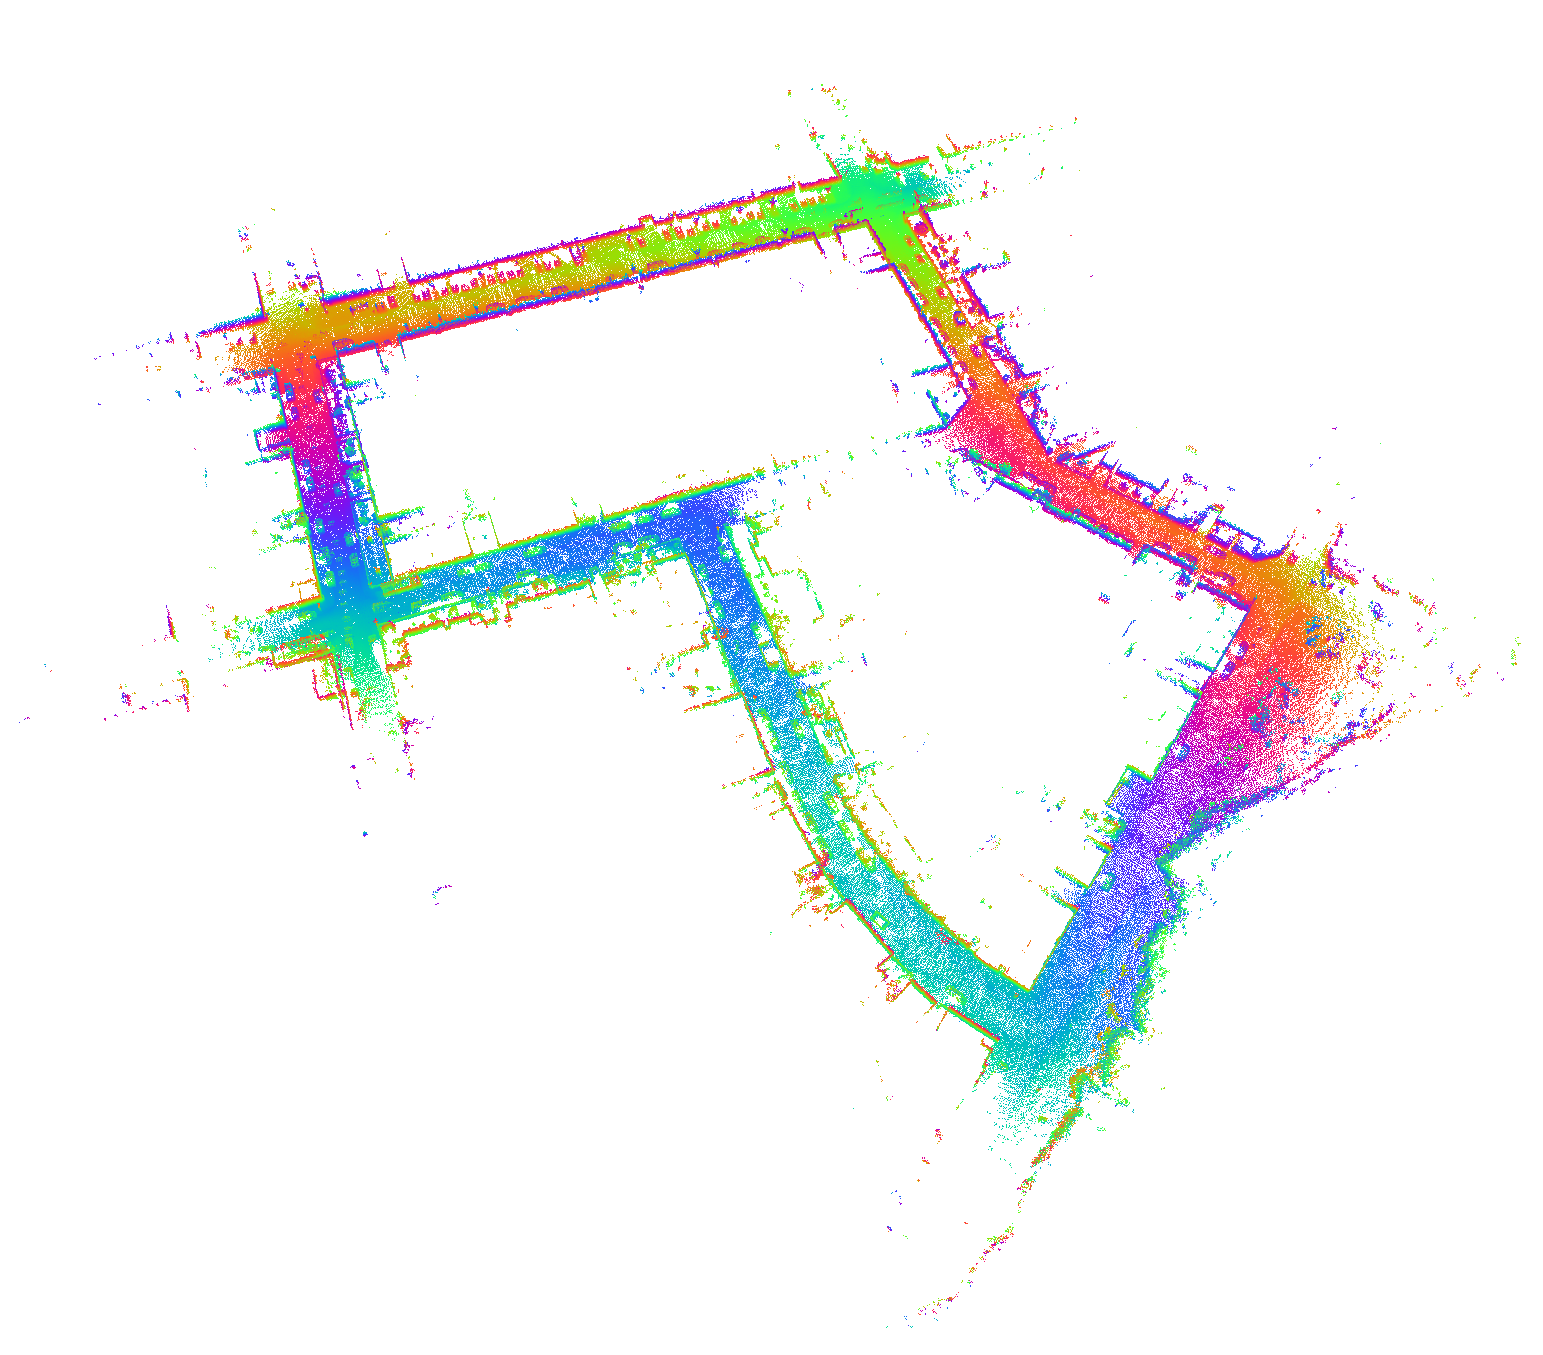
\includegraphics{figs/context/kitty_scan.png}
	\caption{Example of a metropolitan LiDAR point cloud in the SemanticKITTi dataset \cite{behley_towards_2021}, composed of a sequence of scans recorded from a vehicle coupled with a Velodyne LiDAR.}
	\label{fig:kitty_scan}
\end{marginfigure}
The vast majority of LiDAR datasets are oriented towards autonomous driving and perception tasks such as classification, semantic segmentation, instance segmentation and tracking of mobile objects \cite{chen_automatic_2022}, using geometrical \cite{behley_towards_2021} and intensity information \cite{tan_toronto-3d_2020}. Most of them record metropolitan environments from a mobile vehicle coupled with a LiDAR, along with visible and infrared cameras in a few case studies \cite{choi_kaist_2018}. On the other hand, aerial LiDAR datasets covering large portions of the Earth's surface are frequently published by governmental institutions at land inventorying portals. Since these are intended to cover large areas, they are acquired from mid-altitude platforms with a density of a few points per squared meter (up to two points according to the United States Geological Survey \cite{us_geological_survey_lidar_2012} and 0.5 points for the Spanish National Plan of Land Observation \cite{instituto_geografico_de_informacion_geografica_pnoa_nodate}). More recently, despite not being frequent, large and denser aerial LiDAR datasets have also been published \cite{varney_dales_2020}. 

Both kinds of datasets, terrestrial and aerial, are required to be annotated in most nowadays DL applications. Previously revised datasets are recorded by real sensors, and therefore, their classification must be performed manually \cite{behley_towards_2021, pan_semanticposs_2020, tan_toronto-3d_2020} or automatized with networks trained with very limited data \cite{wu_squeezesegv2_2019}. Manual labelling induces errors, but another shortcoming is the lack of detail. For example, these are some real datasets and the number of different semantic labels: SemanticKITTI (25) \cite{behley_towards_2021}, nuScenes (23) \cite{caesar_nuscenes_2020}, SemanticPOSS (14) \cite{pan_semanticposs_2020}, Toronto-3D (8) \cite{tan_toronto-3d_2020} and Semantic3D (8) \cite{hackel_semantic3d_2017}. A more complete compilation of open-source Real LiDAR datasets can be found in \cite{cai_survey_2022}. 

\subsubsection{Motivation of synthetic LiDAR simulation}

LiDAR sensors are expensive imagers that require mobile platforms to generate the mapping of the target scene in a single step, or static platforms producing multiple scans that must be later joined using overlapping features. The former is more prohibitive, while the latter is typically more time-consuming. On the other hand, LiDAR simulators are much more cost- and time-efficient once the emulation challenge has been resolved, which is neither trivial nor efficient to address. Furthermore, it avoids carrying out fieldwork to generate massive datasets and enables optimizing operations with real LiDAR sensors \cite{mohan_robust_2019, li_3d_2022}. Instead of performing scans on real-world scenarios, simulations are performed over synthetic models that can be annotated with any level of detail. Thus, these can feed the resulting point cloud with ground-truth data concerning a wide range of attributes, from normal vectors to semantic annotations. 

There are multiple applications of LiDAR simulations, along with their corresponding research niches. From a hardware perspective, some simulators are focused on the design, validation and calibration of LiDAR sensors \cite{lee_validation_2020}. Their objective is to detect and reduce errors in the scanning, both systematic and random. There are also simulators focused on the optimization of scanning processes \cite{iqbal_simulation_2020, westling_simtreels_2020}, such as the integration of LiDAR data into enhanced and synthetic vision systems \cite{peinecke_lidar_2008}. From a software perspective, one of the most popular research topics is autonomous driving \cite{fang_augmented_2020, li_deep_2020} and navigation \cite{manivasagam_lidarsim_2020}. Most of these methods, especially those based on Deep Learning, benefit significantly from synthetic data. 

Beyond generic research purposes, including teaching and learning, there are systems aimed at the custom configuration of the simulated sensors, including their mounting platform and setup. These simulators typically allow the user to fine-tune all the parameters needed for a physically-based simulation of the laser beams and the interaction with the virtual environment, where photon mapping, Monte Carlo simulation, and full LiDAR waveform generation are their core foundations \cite{yun_simulation_2019, chen_ole_2020, zohdi_rapid_2020}. These frameworks can simulate multiple scattering of the laser beams, taking into account their propagation through wind-driven rough air-water interface \cite{chen_ole_2020}, or vegetation \cite{yun_simulation_2019, westling_simtreels_2020}. There also exist commercial and open-source software such as LGSVL (LG) \cite{lg_electronics_rd_lab_lgsvl_2021}, Simcenter (Siemens Software) \cite{siemens_simcenter_2021}, and CARLA \cite{dosovitskiy_carla_2017} for generating autonomous driving datasets.

\subsubsection{LiDAR simulation}

The early LiDAR simulators produced graphically feasible LiDAR point clouds \cite{gschwandtner_blensor_2011} by emulating the sensor's FOV, occlusion and beam divergence. LiDAR returns were and yet can be solved with ray-casting \cite{ahn_real-time_2020, zhao_method_2021, bechtold_helios_2016} within annotated environments. Remark that ray-cast implies solving impacts of laser emissions through their path (either it is one or five), whereas ray-tracing is reserved for emulating light interaction among surrounding surfaces. The latter represents a physically-based simulation that requires an enormous computation effort and therefore is not yet practical \cite{ahn_real-time_2020}. In recent years, LiDAR simulators have addressed the realistic simulation of geometry returns, the impact of surface properties as well as other environmental conditions. 

Physically-based results have been simulated by including a wide number of errors and limitations. First, Xhao et al. \cite{zhao_method_2021} modelled atmospheric effects such as rain, snow and fog by including signal attenuation and noise. Haider et al. \cite{haider_development_2022} have recently modelled the signal processing within the LiDAR sensor as well as scan patterns to emulate optical losses and defects. Among the cited features, signal attenuation \cite{dosovitskiy_carla_2017, bechtold_helios_2016, hanke_generation_2017}, beam divergence \cite{zhao_method_2021, bechtold_helios_2016, hanke_generation_2017, haider_development_2022} and drop-off in intensity \cite{ahn_real-time_2020} are frequent in the literature. Very few address multiple returns \cite{winiwarter_virtual_2022} despite simulating beam divergence. Other not-that-frequent errors are mirror reflection \cite{ullrich_advances_2019}, motion distortion \cite{chen_analysis_2022}, non-uniform density and distortion of point attributes (colour, intensity, etc.), either as a result of an inappropriate setup \cite{dimitrov_segmentation_2015}, or systematic and random errors \cite{isheil_systematic_2011, fan_error_2015, pandzic_error_2017}. Random errors depend on aspects like the signal-to-noise ratio of the received signal, the accuracy of the electronics (including again the INS and the GPS), the divergence of the laser beams (jittering) and their wavelength, as well as the reflectivity of the objects. Instead of physically emulating these features, previous work has also assessed to deviate ideal synthetic LiDAR point cloud with Deep Learning \cite{manivasagam_lidarsim_2020, xiao_synlidar_2021, guillard_learning_2022}. The leveraging of real LiDAR and synthetic point clouds has also been investigated by mixing scanned urban scenarios and scanned synthetic objects \cite{manivasagam_lidarsim_2020}. Nonetheless, annotation and ground-truth shortcoming remains when leveraging both kinds of data.

Most of these simulators are focused on land scans, while aerial LiDAR has barely been addressed  \cite{winiwarter_virtual_2022}. Westling et al. \cite{westling_simtreels_2020} also included aerial scanning as an unrealistic extension of TLS scans.

Material properties are typically limited to target reflectance regardless of the sensor wavelength \cite{chen_analysis_2022, gschwandtner_blensor_2011, zohdi_rapid_2020}, using phenomenological BRDFs such as Oren-Nayar, Lambertian and Blinn-Phong \cite{chen_analysis_2022}. Other studies use diffuse, specular and transmissive properties acquired from commercial frameworks, such as CarMaker \cite{haider_development_2022}. Intensity has also been simulated with DL for LiDAR data represented with images instead of points \cite{vacek_learning_2022, xiao_synlidar_2021}. However, these networks are conditioned to the learning data and thus to the observed lighting conditions and materials. 

\subsubsection{Time efficiency}

Most studies omit the implementation of LiDAR emulators concerning time efficiency, whereas DL-based approaches are constrained to the calculation time of the network. To the best of our knowledge, only Peinecke et al. \cite{peinecke_lidar_2008} assessed a GPU-based simulation in OpenGL. Furthermore, the efficient semantic labelling and generation of synthetic environments have been poorly addressed, including the annotation of virtual scenes comprising CAD models. Accuracy is also relevant to the simulation since previous work has managed to rapidly solve LiDAR with depth buffers \cite{su_simulation_2019, fang_augmented_2020, manivasagam_lidarsim_2020}. However, these images depict the scene depth with a limited colourimetric resolution, and thus, the resulting geometry may lack precision. Furthermore, the simulation LOD is conditioned to the depth buffer dimensionality and pixel size.

\section{Optimization of LiDAR scans in indoor environments}

\subsection{Motivation} 

LiDAR is widespread in the construction industry for the tracking of building progress by enabling the acquisition of the environment geometry in a precise and highly detailed way. Instead of polygonal meshes, a discretized representation of buildings is given by point clouds. To achieve this goal, Terrestrial Laser Scanning (TLS) is increasingly being used to collect large sets of building data \cite{pandzic_error_2017}. This technology can be applied to a wide range of applications, including building inspections \cite{shariq_revolutionising_2020}, monitoring of natural environments (landform dynamics \cite{guisado-pintado_3d_2019}, ecological resilience \cite{mitasova_geospatial_2010}, etc.), autonomous driving \cite{kuutti_survey_2021} or preservation of cultural heritage \cite{banfi_integration_2019, ham_phased_2020, andriasyan_point_2020}, among others. Besides terrestrial scanners, LiDAR technology presents multiple variants according to their capabilities (range, spatial resolution and covering, etc.) and the platform from which they are operated (Airborne (ALS), Backpack-mounted (BMLS), Mobile Mapping Systems (MMS), Terrestrial (TLS), Satellite (SLS), etc.) \cite{poux_smart_2019, warchol_concept_2019}. 

Some of the main challenges of TLS in the surveying of 3D facilities are the occlusion and range limitations \cite{soudarissanane_optimizing_2012}. Consequently, appropriate planning of TLS scans is necessary in order to 1) minimize the number of different acquisition points, 2) generate a uniformly dense point cloud, and 3) reduce the occlusion from scene objects. These three objectives are equally influenced by the configuration and placement of the scanner. On the other hand, periodic scanning and monitoring of buildings are especially relevant for digitized representations, such as the widely known Building Information Modeling (BIM) \cite{macher_point_2017}. They encode characteristics of a building, including 3D design drawings, materials, costs and safety specifications \cite{patraucean_state_2015}, and provide an interface for the management of 4D applications. Together with TLS, it allows the monitoring of continuously evolving buildings to preserve cultural heritage, track its current state and maintain repair records \cite{rocha_scan--bim_2020, andriasyan_point_2020, moyano_bringing_2020, ham_phased_2020}. However, the monitoring of buildings over time is time-consuming, especially in dynamic environments. Also, TLS surveys generate multiple point clouds that need to be fused either by placing target marks \cite{gollob_comparison_2020} or by estimating the rigid transformation that minimizes the distance among overlapping point clouds. In order to speed up this acquisition task, the development of tools for the planning of TLS surveys plays a key role.

\subsection{Planning for Scanning}

The Planning for Scanning (P4S) has previously been addressed using a wide range of environments and techniques. If the number of target locations is known, then the selection of an optimum set is also known as the NP-complete set-coverage problem \cite{li_probability_2021, mohamadi_efficient_2021, roostapour_pareto_2022}. Previous research can be categorized according to the input environment: model-based or non-model-based (discovered as being explored). The latter is mainly applied to robotic applications whose environment is unknown \cite{potthast_probabilistic_2014}. Otherwise, input scenarios are either defined as 2D or 3D models, with 2D representations being cross-sections of buildings \cite{giorgini_sensor-based_2019}. These 2D-based solutions present lower computational complexity and are frequently solved following an iterative selection of viewpoints (Next Best View; NBV) or guided by heuristic algorithms \cite{aryan_planning_2021}. The main drawback of these algorithms is that they do not consider the details underneath complex buildings. Instead, they are focused on 2D sketches composed of wall edges. 3D-based approaches are far more complex and guided by metrics that allow filtering and ordering space locations. Despite this, the exploration of 3D buildings is also approached with heuristics and NBV. However, the high latency frequently leads to simplifications based on voxelizations \cite{wakisaka_optimal_2019}, Axis-Aligned Bounding Boxes (AABB) and Object-Oriented Bounding Boxes (OOBB) \cite{li_3d_2022}. 2.5D models, such as Digital Surface Models (DSM), have also been investigated similarly to 2D environments \cite{starek_viewshed_2020}.

\subsection{Metaheuristics}

Heuristics are the most frequent solver in P4S. Although they do not provide optimal solutions, they are proven good enough to cover environments with minimum scanning locations. Among heuristics, the Greedy algorithm has been extensively investigated \cite{zhang_rapid_2016, giorgini_sensor-based_2019, heidari_mozaffar_optimal_2016}, followed by Simulated Annealing (SA) \cite{chen_indoor_2018}, Genetic Algorithms (GA) \cite{jia_comparison_2017}, Particle Swarm Optimization \cite{jia_comparison_2017} and Integer Programming \cite{wakisaka_optimal_2019}. Greedy algorithms are based on the iterative selection of locations, according to an objective function. Other Greedy variations weight the locations using a visibility score \cite{jia_comparison_2017}, while others are followed by SA \cite{latimer_sensor_2004}, or optimized with Divide and Conquer (D\&C) \cite{zhang_rapid_2016}. Instead of providing an automatic pipeline, \cite{ahn_interactive_2016} proposed an interactive semi-automatic system.

\begin{figure}[!ht]
	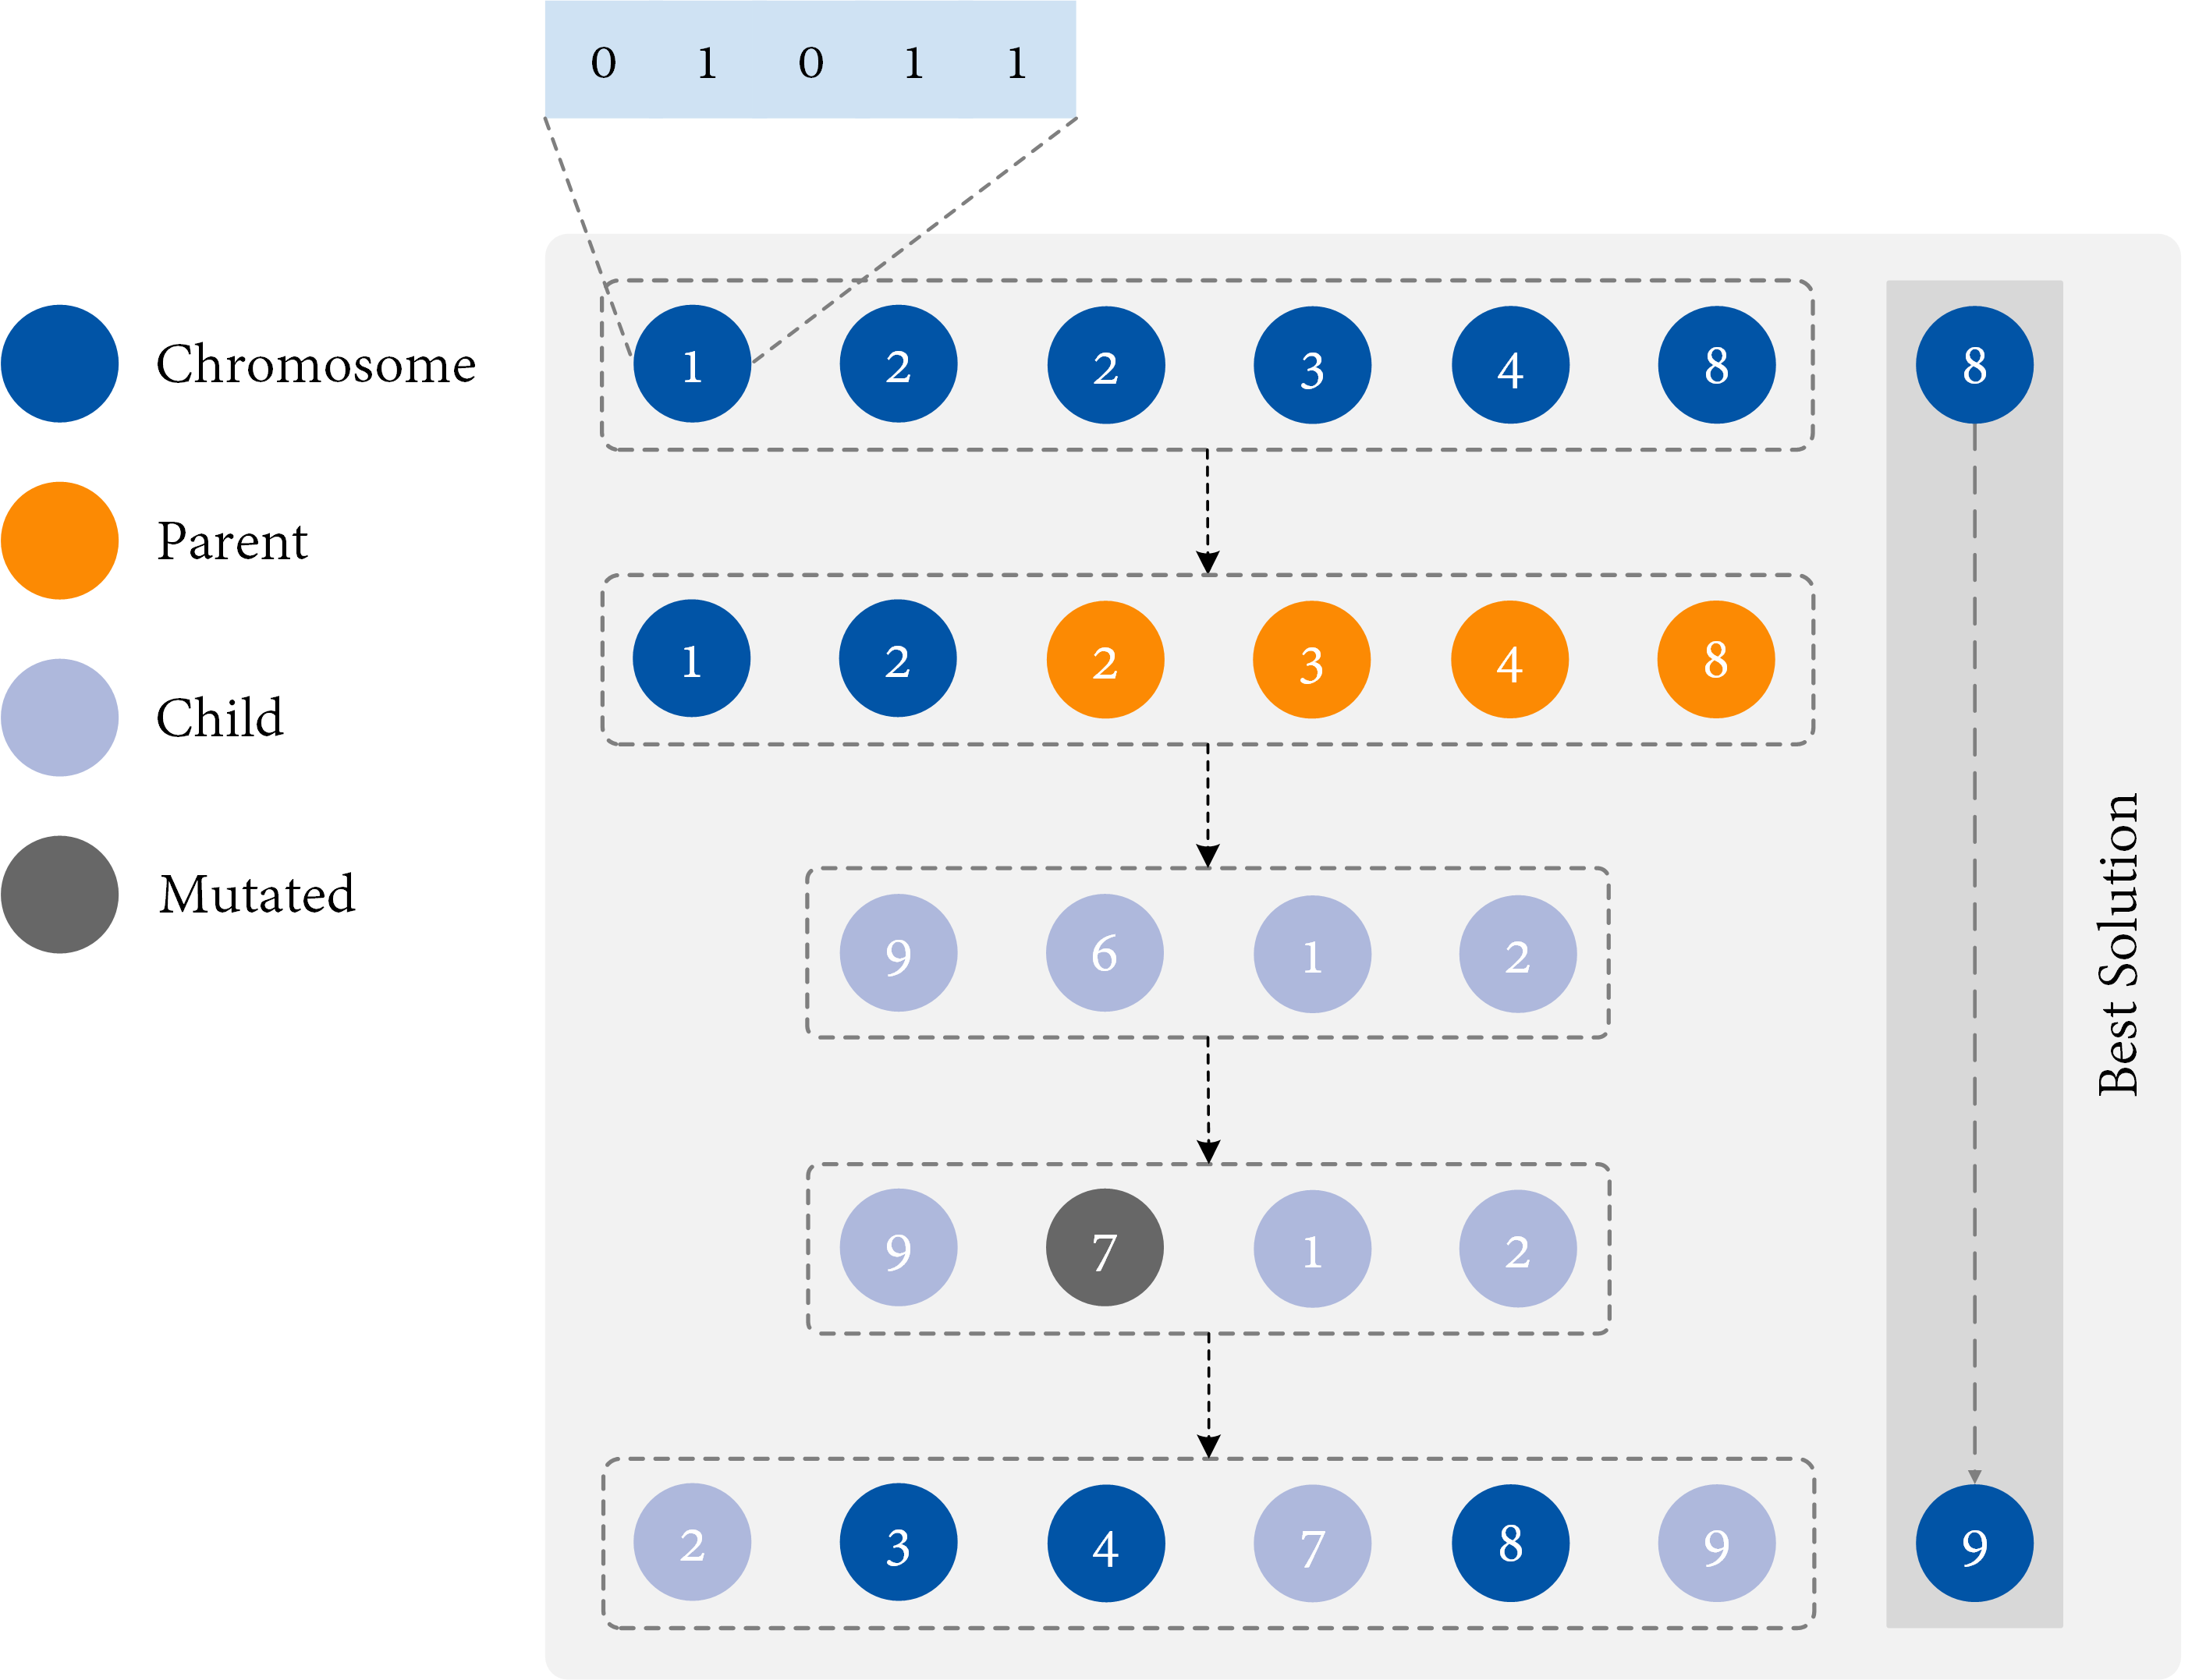
\includegraphics[width=\linewidth]{figs/context/genetic_algorithm.png}
	\caption{Pre-calibration of sensors helps on the projection of multi-source images over a point cloud.}
    \label{fig:genetic_algorithm}
\end{figure}

Heuristic solvers are guided by objective functions measuring the quality of achieved solutions. To evaluate this, four metrics are frequently used in previous work \cite{li_3d_2022, aryan_planning_2021}: Level of Detail (LOD), Level of Accuracy (LOA), Level of Overlap (LOO) and Level of Coverage (LOC). LOD refers to the point cloud resolution, LOA measures the quality of LiDAR returns, as higher distances and angles deteriorate the quality of the measurements \cite{ aryan_planning_2021}, LOO refers to the overlapping area among point clouds so that TLS scans can be joined with rigid transformation estimations, e.g., Iterative Closest Point (ICP), and LOC refers to the number of polygons reached by scans. Thus, the optimization is constrained to limitations concerning range and angles. 

Research on heuristics in 3D is also frequent in the literature, though they are mostly linked to path planning \cite{pehlivanoglu_enhanced_2021} and the selection of subsets \cite{roberge_parallel_2021, pehlivanoglu_enhanced_2021}. However, the number of scans for P4S to meet the required quality is unknown within a non-finite 3D space. The set of possible solutions is narrowed either by selecting random locations \cite{chen_indoor_2018} or sampling the environment as a 2D grid \cite{starek_viewshed_2020, giorgini_sensor-based_2019, jia_comparison_2017}. For uniform subdivisions, the level of detail of the tessellation is a key factor with regard to response time. Coarse subdivisions present lower latency, though they are prone to yield far from optimal solutions. \cite{starek_viewshed_2020} enhances initial locations by applying minor translations while assessing their quality through an objective function, whereas \cite{soudarissanane_optimizing_2012} improves the sampling by increasing the grid subdivisions, at the expense of higher response time. For 3D locations, \cite{starek_viewshed_2020} describes a simulating annealing procedure to transform uniformly sampled points into a surrounding location that improves the covering metric. \cite{kim_placement_2020} finds the optimum LiDAR position over an autonomous vehicle through a Genetic Algorithm (GA). For that purpose, this work utilizes the specifications of commercial LiDARs to compute the occupancy grid of sensor locations, defined as a discretized $360^\circ$ map represented by several views acquiring the coverage region and dead zones. Beyond theoretical/simulation approaches, multiple studies focus on evaluating the set-up of several sensors, concerning height, angles and location in autonomous driving \cite{pereira_self_2016, veronese_accurate_2018}. 

Once locations are locally optimized, they are processed as a classic set-coverage problem \cite{soudarissanane_optimizing_2012}. Recent research has solved this with GA, using different operators and configurations \cite{wang_solving_2018, roostapour_pareto_2022, mohamadi_efficient_2021}. Local searches \cite{li_probability_2021} and other nature-inspired heuristics \cite{islambouli_optimized_2019} are also reviewed. Despite heuristics being allowed to solve hard problems with optimal or nearly optimal solutions, these pose on their efficiency. Previous studies regarding P4S required hours, even days, to determine the optimal scanning configuration in 3D environments. Even 2D-based approaches suffer from high latency \cite{giorgini_sensor-based_2019} if they are implemented sequentially. Thus, multi-core and GPU-based algorithms offer a huge improvement in the response time, reducing it to a few seconds or minutes \cite{giorgini_sensor-based_2019, wang_solving_2018, roberge_parallel_2021}. 

\subsection{Thermography}



\section{Analysis of Remote sensing data}

\subsection{Vineyard phenotyping}

Deep Learning methods have recently become the preferred approach for classifying hyperspectral imagery. However, earlier techniques relied on comparing the acquired data to reference reflectance shapes that were ideally measured in a laboratory. The primary objective of these methods was to measure the similarity between labelled and unlabelled spectral shapes. Spectral libraries, containing data measured from a spectrometer, were used for this purpose. For instance, \cite{kokaly_usgs_2017}, \cite{dutta_characterizing_2017}, and \cite{matusik_data-driven_2003} provided spectral libraries for minerals, trees, and daily surfaces, respectively. These methods varied from the widely used Euclidean distance to more sophisticated techniques such as Spectral Angle Matching (SAM), Cross-Correlogram Spectral Matching (CCSM), and probabilistic approaches like Spectral Information Divergence (SID) \cite{pu_hyperspectral_2017}. Among these techniques, SID and CCSM have been found to perform better in mineral classification from Aviris data. Similarly, \cite{van_der_meer_effectiveness_2006} proved that SAM introduced much more confusion than SID and Spectral Correlation Matching (SCM) in a case study of mineral classification. SAM has the advantage of being invariant to different scales, making it useful for heterogeneous acquisition devices and conditions. Other techniques derived from SAM include Spectral Correlation Angle (SCA), based on the Pearson correlation coefficient, and Spectral Gradient Angle (SGA) \cite{ren_novel_2022}. In addition to similarity, angular and probabilistic measures, the literature describes error and colourimetric methods. The former group includes the widely used Mean Square Error (MSE), Root Mean Square Error (RMSE), Mean Relative Absolute Error (MRAE), Back-Projection MRAE (BPMRAE) and the Peak Signal-to-Noise Ratio (PSNR) \cite{agarla_analysis_2021}. More recently, \cite{kumar_new_2021} introduced three new metrics (Dice Spectral Similarity Coefficient (DSSC), Kumar–Johnson Spectral Similarity Coefficient (KJSSC), and a hybrid of the previous, KJDSSC$_{\textit{tan}}$) that outperformed traditional techniques on mineral and vegetation classification.

Colourimetric measures involve measuring distance in various colour spaces, such as pro-Lab. \cite{agarla_analysis_2021} have compared all these techniques to assess their correlation and determine the most significant ones. Additionally, spectral derivatives, which are finitely approximated considering the previous spectral sample and wavelength distance, are used to remove or compress illumination variations resulting from acquisition conditions \cite{fernandes_grapevine_2019, pu_hyperspectral_2017}. These techniques are still applied when the reflectance profile of different materials exhibits notable variations. Furthermore, semi-automatic classification methods have been reviewed for situations where classification involves only a few labels. For instance, \cite{ahmed_applied_2021} used Principal Component Analysis (PCA) to extract features from multispectral imagery and proposed a vegetation index to label different trees. \cite{padua_monitoring_2020} described similar work on classifying chestnuts with phytosanitary problems using two new indices: ExNIR and ExRE, where Ex refers to Excess. However, these techniques are not suitable for differentiating a significant number of vineyard varieties since they all exhibit similar shapes. We refer the reader to \cite{shanmugam_spectral_2014} for an in-depth revision of spectral matching and attributes conditioning the construction of spectral libraries.

\textbf{Hyperspectral transformation and feature extraction}. In this section, we discuss the transformations that facilitate classification using traditional methods. Due to the extensive coverage of land by satellite imagery, it is uncommon for hyperspectral pixels to depict the spectral signature of a single material. Therefore, there is a prevalent topic in the hyperspectral literature, which involves breaking down the acquired Earth's surfaces by analyzing the hyperspectral images. The problem is illustrated with $\rho = \textit{MF} + \epsilon$, where $M$ is the spectral signature of different materials, $F$ is the weight, $\epsilon$ is an additive noise vector and $\rho$ is an $L \times 1$ matrix where $L$ is the number of bands. Hence, the difficulty of finding a solution to $M$ and $F$ is lowered if $M$ is fixed, i.e., the end-member signatures are known. The Multiple end-member spectral mixture analysis (MESMA) was the initial approach taken,
followed by the Mixture-Tuned Matching Filtering Technique (MTMF), which eliminates the need to know end members in advance. This approach was further refined with the Constrained Energy Minimization (CEM) method, which effectively suppresses undesired background signatures.

The current state-of-the-art techniques for Linear Mixture Models (LMM) can be categorized based on their dependency on libraries. Additionally, the level of supervision and computational cost also determines the classification of these techniques. The taxonomy of methods, as described by \cite{borsoi_spectral_2021}, varies depending on these factors. For instance, Bayesian methods and Local unmixing do not necessitate the need for known end-member signatures, although Bayesian methods are less supervised and more time-intensive. Besides MESMA, other proposed methods that require spectral signatures are based on Artificial Intelligence techniques such as Machine Learning and Fuzzy unmixing. The latter is less supervised but more time-consuming. In recent years, interest in Deep Learning (DL) has grown, with techniques such as autoencoders, Convolutional Neural Networks (CNN), and Generative Adversarial Networks (GAN) are being utilized for training with synthetic data \cite{bhatt_deep_2020}. Nonnegative matrix factorization (NNMF) has also attracted attention as it can extract sparse and interpretable features \cite{hruska_machine_2018}. Recently, the incorporation of spatial information into hyperspectral unmixing has been investigated \cite{shi_incorporating_2014}. This involves considering the surrounding pixels using kernels of varying sizes and shapes, such as squared, cross, or adaptive. Weights can also be assigned based on the distance to the centre and the measured similarity using functions like SID, SAM, Euclidean distance, etc. Current state-of-the-art methods, such as NNMF, have been combined with spectral information \cite{zhang_spectral-spatial_2022}.

Besides discerning materials, the results of Hyperspectral Imaging (HSI) present a large number of layers that can be either narrowed or transformed, as many of them present a high correlation. Otherwise, the large dimensionality of HSI data leads neural networks and other classification algorithms to be hugely complex. Accordingly, the most frequent projection method is Principal Component Analysis (PCA) \cite{jiang_rapid_2022, shenming_new_2022, lu_hyperspectral_2022}, which projects an HSI cube of size $X \times Y \times \lambda$ into $DB$, where $D$ has a size of $X \times Y \times F$, and $B$ is a matrix such as $F \times \lambda$. In this formulation, $F$ is the number of target features \cite{amigo_hyperspectral_2019}. Independent Component Analysis (ICA) is a variation of Principal Component Analysis (PCA) that not only decorrelates data but also identifies normalized basis vectors that are statistically independent \cite{pu_hyperspectral_2017}. Least Discriminant Analysis is another commonly used technique, but it is primarily applied after PCA to increase inter-class and intra-class distance \cite{shenming_new_2022}. In the literature, it is also referred to as Partial Least-Square Discriminant Analysis (PLS-DA), mainly as a classifier rather than a feature selection method.

Instead of projecting features into another space, these can be narrowed into the subset with maximum variance according to the classification labels of HSI samples. There are many techniques in this field, including the Successive Projection Algorithm (SPA), which reduces colinearity in the feature vector. The Competitive Adaptive Reweighted Sampling (CARS) method selects features with Monte-Carlo sampling and iteratively removes those with small absolute regression coefficients. Two-Dimensional Correlation Spectroscopy (2DCS) aims to characterize the similarity of variance in reflectance intensity. \cite{liu_dimension_2019} used the Ruck sensitivity analysis to discard bands with a value below a certain threshold. \cite{agilandeeswari_crop_2022} calculated the band entropy, vegetation index, and water index for wavelength subsets, generating a narrower cube only with bands above three different thresholds. Finally, the work of \cite{santos-rufo_wavelength_2020} presents an in-depth evaluation of methods based on Partial Least Squares (PLS) regression. To this end, HSI data from olive orchards were first narrowed and then classified with LDA and K-Nearest Neighbours (KNN). In conclusion, the Lasso method \cite{friedman_regularization_2010}, as well as Genetic algorithms, \cite{mehmood_review_2012} showed the best performance with LDA. 

Remote sensing data typically contains inherent noise, which means it is rarely used as-is. To address this issue, \cite{gutierrez_--go_2018} used a combination of Standard Normal Variate (SNV) and de-trending to remove the scatter effect. They then smoothed the hyperspectral signature by applying Savitzky-Golay filtering with different step sizes over the first and second derivatives.

\textbf{Classification of hyperspectral imaging with ML and DL}. This section focuses on reviewing studies related to the classification of vineyard varieties using hyperspectral imagery (HSI). Although there are numerous studies on HSI classification, only those relevant to vineyard varieties will be discussed. In addition, state-of-the-art deep learning (DL) networks achieving high accuracy in HSI classification will also be briefly reviewed.

Despite there exists considerable research on segmentation, only a few studies have addressed the classification of vineyard varieties using RGB and multispectral imagery. In these studies, binary masks or grayscale maps were first extracted to distinguish soil, shadows, and vineyards. Clustering, line detection, or machine learning (ML) algorithms and artificial neural networks (ANNs) were then applied to segment vineyard rows \cite{fuentes-penailillo_using_2018, karatzinis_towards_2020, hajjar_vine_2021, padua_monitoring_2020, padua_vineyard_2022, poblete-echeverria_detection_2017}. Geometrical information from depth maps, digital elevation models (DEMs), LiDAR data, and photogrammetric reconstructions were also assessed \cite{kerkech_vine_2020, aguiar_localization_2022, jurado_automatic_2020}. DL approaches for semantic segmentation and skeletonization algorithms were also discussed \cite{kerkech_vine_2020-1, barros_multispectral_2022, nolan_automated_2015}. Further insight into this field is provided in \cite{li_performance_2020}. 

The classification of different vineyard varieties has been previously achieved with traditional methods and proximal hyperspectral sensing. Samples were selected by manually averaging the variety signature and filtering those with high correlation to such a signature. Support Vector Machine (SVM) and Multilayer Perceptron (MLP) were then trained with k-fold to distinguish thirty varieties, with the latter obtaining better results. \cite{kicherer_phenoliner_2017} also presented a land phenotyping platform that segments grapes from the depth map and discerns between sprayed and non-sprayed leaves. To this end, several learning models were tested: LDA, Partially Least Square (PLS), Radial Basis Function (RBF), MLP and soft-max output layer (PNET), with RBF and PLS showing the best results. Besides phenotyping, the following work is aimed at detecting diseases \cite{nguyen_early_2021, bendel_detection_2020, bendel_evaluating_2020} and plagues \cite{mendes_vineinspector_2022}. However, these applications formulate a binary problem where signatures of distinct classes are significantly different regarding scale \cite{bendel_detection_2020} and shape \cite{bendel_detection_2020}. Despite this, previous learning models are also implemented (MLP, RBF, PLS and LDA) and almost achieved the perfect discrimination performance \cite{bendel_evaluating_2020}. \cite{nguyen_early_2021} conducted a study similar to ours, where they attempted to differentiate healthy and infected leaves with a comparable spectral signature. However, their data was obtained from land, and they used the flattened layer of 2D and 3D convolutional networks as input for Random Forest (RF) and SVM algorithms. They found that combining PCA reduction (50 features) and RF resulted in the best performance (97\%), and RF improved SVM classification regardless of data reduction. Additionally, ML and DL techniques have been extensively applied to various crops, such as maize, sugarcane, rice, and bread wheat, using both satellite and proximal imaging. Transfer learning, attention-based, and residual models are commonly used in the literature \cite{zhang_classification_2022}. A lightweight CNN composed of several inception blocks was also developed to classify up to 15 plant species \cite{liu_plant_2022}. The authors compared their proposed CNN model to other commonly used models for classifying RGB images, including AlexNet, VGGNet, and GoogLeNet. They found that the best results were achieved using a combination of six RGB and Near Infrared features, with an accuracy of 94.7\%. The use of PCA with only six features achieved an accuracy of 88\%. \cite{nezami_tree_2020} also applied a 3D CNN to classify three tree species using both hyperspectral and visible imaging, as well as canopy height models as input. However, their overall accuracy was below 95\%.

When it comes to DL for the classification of satellite hyperspectral imaging, it is more current than UAV imaging. A standard dataset is available for this purpose, on which several experiments have been conducted. Among them, the top-performing models based on overall accuracy (OA) are discussed below. \cite{moraga_jigsawhsi_2022} presented an Inception-based model with parallel convolutional pipelines of increasing size, achieving near-perfect classification. \cite{chakraborty_spectralnet_2021} proposed the SpectralNet model, which combines wavelet decompositions with a traditional convolutional path (OA: 98.59\%-100\%). \cite{roy_hybridsn_2020} developed HybridSN, which includes both spectral-spatial and spatial feature learning using 3D and 2D convolutional layers (OA: 99.63\%-100\%). \cite{roy_attention-based_2021} later introduced a network based on residual blocks and spectral-spatial attention modules with varying architecture (start, middle and ending ResBlock) (OA: 98.77\%-99.9\%). Lastly, the A-SOP network \cite{xue_attention-based_2021} proposed a module composed of matrix-wise operations that output a second-order pooling from the attention weights, after extracting the first-order features (OA: 98.68\%-100\%). 

Similar to Moraga and Duzgun's work in 2022, the FSKNet model also employs a combination of 2D and 3D convolutional layers with an intermediate separable convolution to reduce training latency while achieving comparable overall accuracy results. The FSKNet model achieves an OA above 99\% with significantly fewer parameters and a shorter training time. This work focuses on single output classification, where the output is either hot-encoded or given as a single value. However, other approaches have gained attention, such as contrastive learning and multi-instance segmentation, which propose outputs of higher dimensionality. \cite{zhu_spectral-spatial-dependent_2021} investigated pixel-wise classification of HSI patches using semantic segmentation, using the popular U-Net architecture with additional convolutional LSTM and attention-based mechanisms. \cite{xin_convolution_2022} used transformers to independently encode spatial and spectral features and then combine them. Contrastive learning has also been used to address the lack of labelled datasets, where HSI patches and 1D data are jointly used during training so that the network learns by comparing pairs of samples \cite{guan_spatial-spectral_2022}. Finally, \cite{meerdink_multitarget_2022} accurately labelled HSI with multi-instance learning by creating bags of samples with distinct labels.

\subsection{Inspection of archaeological remains}

Unmanned Aerial Systems (UAS) have been widely applied in archaeological fieldwork during the last decade \cite{campana_drones_2017} and data obtained from aerial and satellite imagery is well established for analyzing archaeological landscapes \cite{waagen_new_2019}. Among them, the results of UAS can be used to generate orthophotos and Digital Elevation Models (DEM) that facilitate the observation of archaeological marks and microreliefs as proxy indicators of the presence of buried remains \cite{pecci_archaeology_2016, dubbini_digital_2016}. Furthermore, the archaeological remains are frequently located in natural landscapes barely accessible by humans with irregular features. As a result, UAS-based solutions have been applied to 3D reconstructions as an efficient technology that covers large and inaccessible areas. 

The preservation of cultural heritage has recently benefited from the use of high-resolution digital cameras that allow the reconstruction of a scenario with high precision. Aerial images acquired from drones not only allow us to generate 3D models using photogrammetric and SfM techniques but also to obtain information beyond the visible range depending on the coupled sensors. Aerial thermographic imaging has been extensively studied in archaeology as an alternative to visible sensors \cite{casana_archaeological_2017, brooke_thermal_2018, mcleester_detecting_2018, salgado_carmona_assessing_2020}, since it allows recording the radiation emitted from object surfaces, either it proceeds from the object itself or surrounding objects \cite{vollmer_infrared_2017}. Therefore, it is possible to detect buried archaeological remains through thermal imagery whether heat transfer occurs \cite{casana_archaeological_2017}. Nevertheless, their detection is enhanced if (1) there exists a significant thermal contrast between the background and relevant features, (2) the UAS flight is performed at specific day intervals where the contrast of ambient temperature and sunlight radiation is higher, and (3), buried features are close to the surface. Despite thermal orthomosaics of the surveyed environment being mostly sufficient to reveal artefacts \cite{mcleester_detecting_2018, salgado_carmona_assessing_2020}, they can be augmented by modelling thermal reconstructions as a 3D surface. However, consumer-grade thermal cameras present low resolution (typically 640x512 or 640x480 pixels) that limits the capability of conventional photogrammetry to generate dense and large thermal point clouds required to analyze the archaeological site \cite{javadnejad_photogrammetric_2020}. Previous work has achieved the fusion of thermography and 3D data, either from LiDAR or photogrammetry \cite{patrucco_3d_2022}, though it was applied to land surveys and the inspection of façades.

In contrast to thermal imagery, visible sensors acquire images of higher resolution, enabling the estimation of larger and more dense point clouds. However, RGB point clouds can be used as a constrained data source to map thermographic information, thus taking advantage of their spatial characteristics. For that purpose, the relative difference between visible and thermal imaging sensors needs to be estimated in order to project 3D points into TIR images. The calibration of both sensors can be performed before the flight, by detecting key points in checkerboards or similar patterns \cite{adan_towards_2020, javadnejad_photogrammetric_2020}, or afterwards, by registering co-acquired images \cite{javadnejad_photogrammetric_2020}. Although multiple projection algorithms are described in the literature, this range of methods outperforms others based on the Iterative Closest Point (ICP) \cite{webster_three-dimensional_2018} or solely based on SfM reconstruction \cite{gonzalez_thermal_2019, grechi_3d_2021}, both in terms of precision and density. 






